%===========================================================
\chapter{Predictive Modelling, Constrained Optimisation and Biological Interpretation}
\label{chap:model_training_evaluation}
%===========================================================

%-----------------------------------------------------------
\section{From Robust Feature Selection to Predictive Modelling}
%-----------------------------------------------------------

Chapter~\ref{chap:feature_selection} established a statistically stable and 
structurally diversified CpG panel of fixed cardinality ($K = 5{,}000$) for 
each dataset, integrating variability screening, biologically weighted stability 
selection, redundancy pruning, and genomic diversification. The inter-dataset 
evaluation of Section~\ref{sec:inter_dataset_fs} further revealed that cross-cohort replicability is 
partial and asymmetric: GSE69914 and GSE225845 share a concordant drift 
orientation and support bidirectional zero-shot transfer, whereas GSE287331 
exhibits a systematically inverted drift axis, yielding sub-random transfer 
performance against both partner cohorts.
The objectives of this chapter are threefold. First, intra-dataset 
classification performance is quantified to verify whether the selected panels 
support accurate Normal--Adjacent discrimination within each cohort; a linear 
Support Vector Machine is adopted for GSE225845 and GSE287331, and a 
$k$-Nearest Neighbours classifier for GSE69914 to probe the degree of linear 
separability. Second, cross-dataset transferability is examined under a 
zero-leakage design — training on one cohort and evaluating directly on another 
— to quantify how well the inferred epigenetic drift axis generalises across 
independent cohorts, and whether performance degradation is systematically 
associated with the directional concordance structure of 
Chapter~\ref{chap:feature_selection}. Third, a constrained combinatorial 
compression step derives a compact 50-CpG subset via mixed-integer linear 
programming, investigating whether predictive structure and biological diversity 
can be jointly preserved under severe dimensional reduction.
The biological coherence of the compressed panels is then evaluated through 
CpG-to-gene mapping, cross-referenced against the COSMIC Cancer Gene Census 
(CGC, version 103, GRCh38)~\cite{sondka2018cosmic,cosmic_cgc_v103}, and 
pathway-level enrichment analysis — closing the loop between statistical 
discrimination and functional relevance. The limitations that emerge, in 
particular the failure of linear $\Delta\beta$ signatures to generalise across 
cohorts with divergent drift orientations, directly motivate the 
representation-learning approach of Chapter~\ref{chap:multi_cohort_integration}.

%-----------------------------------------------------------
\section{Supervised Learning Framework}
%-----------------------------------------------------------

Each dataset is restricted to its corresponding $K = 5{,}000$
CpG panel and two baseline classifiers are evaluated
independently within each cohort: a linear Support Vector
Machine for GSE225845 and GSE287331, and a $k$-Nearest
Neighbours for GSE69914 to probe linear separability.
The primary aim is not to maximise predictive performance
but to quantify the discriminative content encoded in the
selected panels.


%-----------------------------------------------------------
\subsection{Intra-Dataset Supervised Modelling}
\label{sec:intra_modelling}
%-----------------------------------------------------------

\paragraph{Data partitioning and leakage control}

For each dataset, samples are partitioned into stratified
training and test sets under an 80/20 split, preserving the
Normal--Adjacent class proportions. Feature selection was
performed strictly within training folds in
Chapter~\ref{chap:feature_selection}, so no information from
the held-out set influences the choice of CpGs. Standardisation
is fitted exclusively on the training partition and applied
without re-estimation to the test set, ensuring complete
leakage control throughout the pipeline.

\paragraph{Linear Support Vector Machine}

A linear Support Vector Machine (SVM) is adopted as the
primary classifier for GSE225845 and
GSE287331~\cite{cortes1995svm}. This choice is motivated by
two reasons. First, the feature space is high-dimensional
relative to sample size, a regime where linear models exhibit
strong empirical performance and avoid the curse of
dimensionality affecting kernel methods. Second, the linear
decision boundary admits a direct geometric interpretation
along the epigenetic drift axis: the weight vector $w$
identifies the methylation direction most separating Normal
and Adjacent tissues, enabling hyperplane comparison across
cohorts in the cross-dataset analysis of
Section~\ref{sec:cross_dataset}.
\noindent Given training data $\{(x_i, y_i)\}_{i=1}^n$ with
$x_i \in \mathbb{R}^p$ and $y_i \in \{-1,+1\}$, the soft-margin
primal formulation is:

\begin{equation}
\min_{w,b,\xi} \quad
\frac{1}{2}\lVert w\rVert^2 + C \sum_{i=1}^n \xi_i
\quad\text{s.t.}\quad
y_i(w^\top x_i + b) \ge 1 - \xi_i,\ \xi_i \ge 0.
\end{equation}

\noindent The decision function is $f(x) = w^\top x + b$, with class
assignment given by $\mathrm{sign}(f(x))$. All models are
trained on standardised $M$-values with fixed hyperparameters
($C = 0.5$, $\texttt{max\_iter} = 10{,}000$), deliberately
avoiding data-driven tuning to keep the evaluation as a
measure of the panel's intrinsic discriminative content rather
than of classifier optimisation.

\paragraph{$k$-Nearest Neighbours (GSE69914 only)}

For GSE69914, a $k$-Nearest Neighbours classifier is
introduced as a local,
non-parametric baseline~\cite{cover1967nn}. Its inclusion
serves a specific diagnostic purpose: it is possible to assess whether the discriminative
signal in GSE69914 is linearly structured or whether it
resides in local manifold geometry. For a query $x$, let
$\mathcal{N}_k(x)$ denote the set of the $k$ closest training
samples under Euclidean distance; the predicted label is:

\begin{equation}
\hat{y}(x) = \operatorname{mode}\{y_i :\ x_i \in \mathcal{N}_k(x)\}.
\end{equation}

\noindent The method is applied on standardised features with fixed $k = 5$.

\paragraph{Performance metrics}

Classification performance is evaluated through a complementary set of metrics
designed to provide a complete picture under potential class imbalance. The
Area Under the ROC Curve (AUC), defined in
Chapter~\ref{chap:feature_selection}, serves as the primary threshold-free
discriminability measure.
To assess performance independently of class distribution, two summary scalar
indices are adopted. \emph{Balanced accuracy} ($\mathrm{BAcc}$) is defined as
the arithmetic mean of sensitivity and specificity:
\begin{equation}
\mathrm{BAcc} = \frac{1}{2}\!\left(
  \frac{\mathrm{TP}}{\mathrm{TP}+\mathrm{FN}} +
  \frac{\mathrm{TN}}{\mathrm{TN}+\mathrm{FP}}
\right).
\end{equation}
The \emph{Matthews Correlation Coefficient} (MCC) provides a single scalar
that accounts simultaneously for all four entries of the confusion matrix,
making it particularly robust when class sizes differ substantially:
\begin{equation}
\mathrm{MCC} =
\frac{\mathrm{TP}\cdot\mathrm{TN} - \mathrm{FP}\cdot\mathrm{FN}}
{\sqrt{(\mathrm{TP}+\mathrm{FP})(\mathrm{TP}+\mathrm{FN})
       (\mathrm{TN}+\mathrm{FP})(\mathrm{TN}+\mathrm{FN})}}.
\end{equation}

\noindent At the operating threshold, performance is further characterised through
precision~$p$ — the fraction of positive predictions that are correct —
recall~$r$ — the fraction of true positives retrieved — and their harmonic
mean, the F1-score, which provides a single balanced summary of the
precision--recall trade-off:
\begin{equation}
p = \frac{\mathrm{TP}}{\mathrm{TP}+\mathrm{FP}},
\qquad
r = \frac{\mathrm{TP}}{\mathrm{TP}+\mathrm{FN}},
\qquad
\mathrm{F1} = \frac{2\,p\cdot r}{p+r}.
\end{equation}

%-----------------------------------------------------------
\subsection{Cross-Dataset Generalisation Protocol}
\label{sec:cross_dataset}
%-----------------------------------------------------------

The cross-cohort transferability analysis addresses a question
that intra-dataset evaluation cannot answer: whether the
epigenetic drift axis inferred within a single cohort encodes
a portable biological signal or a cohort-specific artefact.
The design is deliberately zero-leakage — no information from
the target dataset enters the training procedure at any stage
— so that performance on the external cohort reflects true
out-of-distribution generalisation rather than any form of
implicit adaptation.

\paragraph{Feature space alignment}

Cross-dataset evaluation requires strict alignment of the
feature space between source and target cohorts. For each
ordered pair $(A, B)$, the CpG panel is restricted to the
intersection of the effective 5,000-CpG sets retained after
intra-dataset feature selection in cohort $A$: only CpGs
present in both datasets and included in the source panel are
considered. Column ordering is explicitly harmonised to ensure
identical feature indexing across matrices, and all
transformations — including the $\beta \to M$ mapping where
required — are applied consistently prior to modelling. No
re-selection, re-ranking, or any other data-driven operation
is performed on the target cohort.

\paragraph{Train-on-$A$ / Test-on-$B$ design}

The classifier is trained exclusively on the training split
of cohort $A$ over the aligned CpG space. Feature
standardisation is fitted on the source training partition
and applied without re-estimation to cohort $B$. Probability
calibration is performed via sigmoid fitting with three-fold
internal cross-validation, entirely within the source training
data, and the resulting calibrated decision function is
evaluated directly on the target cohort. No hyperparameter
tuning, retraining, or distributional adaptation is performed
on $B$ at any stage. This strict separation quantifies true
zero-shot transferability of the learned separating hyperplane.

\paragraph{Evaluation criteria}

Performance is quantified using the same metrics as in the
intra-dataset setting — AUC, balanced accuracy, and MCC —
reported jointly for the internal test split of cohort $A$ and
the external cohort $B$, so that within-cohort and
cross-cohort discrimination can be compared directly.
Degradation in external AUC or balanced accuracy is
interpreted as evidence that the learned separating hyperplane
does not align with the drift structure of the target cohort.
Of particular interest is the case of systematic performance
inversion, examined against the directional concordance
structure documented in Chapter~\ref{chap:feature_selection}:
external performance below random expectation
($\mathrm{AUC} \approx 0.5$) is treated as a signature of
reversed drift orientation rather than of weak shared signal,
a distinction that carries direct methodological implications
for the multi-cohort strategy developed in
Chapter~\ref{chap:multi_cohort_integration}.

%-----------------------------------------------------------
\subsection{Constrained Subset Optimisation via Knapsack Formulation}
\label{sec:knapsack}
%-----------------------------------------------------------

The 5{,}000-CpG panel retains substantial redundancy relative to the intrinsic
dimensionality of the discriminative signal. A further compression step is therefore
introduced with the dual aim of isolating the most informative loci and verifying
whether predictive performance and biological diversity can be jointly preserved
under severe cardinality reduction. The target panel size is fixed at $K = 50$,
corresponding to a 100-fold compression relative to the input set.
The selection problem is cast as a multi-constraint mixed-integer linear programme
(MILP), inspired by the classical $0$--$1$ knapsack problem of~\cite{dantzig1957}
and extended to incorporate structural and biological requirements analogous to
those employed in marker panel design~\cite{wu2016snp,nishiyama2022ilp}. Unlike
the classical single-capacity formulation, the present model couples a composite
statistical objective with eight hard constraints that jointly enforce cardinality,
correlation independence, chromosomal balance, biological-region anchoring,
gene-level linking, per-gene diversity, gene-count diversity,
and methylation directionality.

\paragraph{Decision variables and composite score}

Let $\mathcal{J}$ denote the index set of $|\mathcal{J}| = 5{,}000$ candidate
CpGs retained after feature selection. For each $j \in \mathcal{J}$, a binary
decision variable $x_j \in \{0,1\}$ encodes inclusion in the compressed panel.
Gene-level linking variables $y_g \in \{0,1\}$ indicate whether at least one
CpG annotated to gene $g$ is selected, and enter both the diversification
objective~\eqref{eq:phi} and constraint~\eqref{eq:c5}.
The statistical utility of each locus is summarised by a composite score:
\begin{equation}
\label{eq:score}
  v_j \;=\;
  w_{\mathrm{coef}}\,\tilde{c}_j
  + w_{\Delta M}\,\tilde{d}_j
  + w_{\sigma}\,\tilde{s}_j
  + w_{\mathrm{COSMIC}}\,\mathbf{1}_{\{j \in \mathrm{CGC}\}},
\end{equation}
where $\tilde{c}_j$, $\tilde{d}_j$, and $\tilde{s}_j$ are rank-normalised
components corresponding, respectively, to the SVM coefficient magnitude,
the absolute $\Delta M$ effect size, and the inverse cross-sample standard deviation of M-values on the training set,
such that loci with low baseline variability in Normal tissue receive higher utility; the indicator $\mathbf{1}_{\{j \in \mathrm{CGC}\}}$
confers an additional reward to loci annotated in the COSMIC Cancer Gene
Census~\cite{sondka2018cosmic}.
The normalised diversification functional is defined as:
\begin{equation}
\label{eq:phi}
\hat{\Phi}(x,y) \;=\;
\frac{1}{K(2+\eta)}\left(
\sum_{j:\,\mathrm{prom}(j)} x_j
+ \sum_{j:\,\mathrm{isl}(j)} x_j
+ \eta \sum_{g} y_g
\right),
\end{equation}
where $\mathrm{prom}(j)$ indicates that locus $j$ is promoter-proximal
(TSS200, TSS1500, 1stExon, or 5'UTR), $\mathrm{isl}(j)$ indicates membership
in a CpG island, and $\eta > 0$ weights gene-level richness relative to regional
coverage. The denominator $K(2+\eta)$ normalises $\hat{\Phi}$ to the unit
interval, so that $\mu$ is directly interpretable as the maximum fractional
penalty on the statistical objective.

\paragraph{Complete MILP formulation}

Combining~\eqref{eq:score} with~\eqref{eq:phi}, the full optimisation problem
reads:
\begin{align}
&\underset{x}{\text{max}} \quad
  \sum_{j \in \mathcal{J}} v_j\,x_j + \mu\,\hat{\Phi}(x,y) \notag \\[8pt]
&\text{s.t.} \notag \\[4pt]
&\quad \sum_{j \in \mathcal{J}} x_j = K
   \label{eq:c1}\\[3pt]
&\quad x_i + x_j \le 1
   \qquad \forall\,(i,j):\,|r_{ij}| \ge 0.85
   \label{eq:c2}\\[3pt]
&\quad \sum_{j \in \mathcal{J}_c} x_j \le \delta_{\mathrm{chr}}
   \qquad \forall\, c
   \label{eq:c3}\\[3pt]
&\quad \sum_{j \in \mathcal{J}_A} x_j \ge K_A
   \qquad \text{if } \mathcal{J}_A \neq \emptyset
   \label{eq:c4}\\[3pt]
&\quad x_j \le y_{g(j)}
   \qquad \forall\, j:\, g(j) \neq \emptyset
   \label{eq:c5}\\[3pt]
&\quad \sum_{j:\,g(j)=g} x_j \le \delta_{\max}
   \qquad \forall\, g
   \label{eq:c6}\\[3pt]
&\quad \sum_{g} y_g \ge G_{\min}
   \label{eq:c7}\\[3pt]
&\quad \sum_{j:\,\Delta M_j > 0} x_j \ge h_{\min}
   \label{eq:c8}\\[3pt]
&\quad x_j \in \{0,1\},\quad y_g \in \{0,1\}. \notag
\end{align}

\noindent Each constraint encodes a distinct biological or structural requirement.
Constraint~\eqref{eq:c1} fixes the panel cardinality exactly at $K = 50$.
Constraint~\eqref{eq:c2} prevents the simultaneous selection of locus pairs whose
Spearman correlation satisfies $|r_{ij}| \ge 0.85$, extending the
redundancy-pruning principle of Chapter~\ref{chap:feature_selection} to the
compressed regime. Constraint~\eqref{eq:c3} imposes an absolute ceiling
$\delta_{\mathrm{chr}} = 10$ on the number of loci selected from any single
chromosome, preventing genomic concentration. Constraint~\eqref{eq:c4} enforces
a lower bound $K_A$ on the number of loci drawn from Pool~A --- the biologically
anchored subset of CpG-island-proximal sites identified during feature selection
--- and is active only when $\mathcal{J}_A \neq \emptyset$.
Constraints~\eqref{eq:c5} and~\eqref{eq:c6} jointly govern gene-level diversity:
\eqref{eq:c5} activates the linking variable $y_{g(j)}$ whenever CpG $j$ is
selected, while \eqref{eq:c6} independently caps the number of selected loci per
gene at $\delta_{\max} = 2$, preventing any single locus neighbourhood from
dominating the panel. Constraint~\eqref{eq:c7} imposes a lower bound $G_{\min}$
on the number of distinct genes represented, promoting broad regulatory coverage.
Finally, constraint~\eqref{eq:c8} enforces a minimum count $h_{\min}$ of loci
with positive SVM coefficient, i.e.\ hypermethylated in Adjacent relative to
Normal tissue, preventing polarity collapse towards a purely hypomethylated
solution.

\paragraph{Optimisation strategy and parameter selection}

The scalar $\mu \ge 0$ governs the trade-off between statistical score and
structural diversification. At $\mu = 0$ the problem reduces to a pure
score-maximising knapsack; as $\mu$ increases, the objective increasingly
rewards genomic balance at the expense of discriminative utility. To identify
a stable operating point, $\mu$ is swept over the discrete grid
$\{0,\, 0.05,\, 0.1,\, 0.25,\, 0.5,\, 1.0,\, 2.0\}$ and the resulting
Pareto frontier between $f_1 = \sum_j v_j x_j$ and $f_2 = \hat{\Phi}(x,y)$
is examined. The final value is selected at the empirical knee of this curve,
defined as the point of maximum perpendicular distance from the line connecting
the two frontier endpoints, beyond which marginal gains in diversification no
longer compensate for losses in statistical score. An independent sweep over
$w_{\mathrm{COSMIC}} \in \{0,\, 0.1,\, 0.2,\, 0.3,\, 0.5,\, 0.7,\, 1.0\}$
is subsequently performed at the knee $\mu$, and the value maximising COSMIC
enrichment subject to a tolerance of $0.1\%$ on $f_1$ is retained.
Solution stability across $\mu$ values is assessed by computing the Jaccard
similarity between each solution and the knee-point panel, confirming that the
selected subset is not sensitive to small perturbations of the diversification
weight. Given the moderate input dimensionality ($|\mathcal{J}| = 5{,}000$),
the MILP is solved to certified global optimality using the COIN-OR
Branch-and-Cut (CBC) solver interfaced via the PuLP modelling library, with a
wall-clock time limit of 120 seconds per instance.

%-----------------------------------------------------------
\subsection{Functional and Gene-Level Interpretation}
\label{sec:gene_enrichment}
%-----------------------------------------------------------

Having established the discriminative capacity of the compressed
panels, this subsection examines whether the loci selected
through purely statistical and structural criteria converge
on genes with documented roles in cancer biology. The analysis
proceeds in two stages: CpG-to-gene mapping followed by
over-representation testing against curated pathway databases.

\paragraph{CpG-to-gene mapping and methylation directionality}

Each of the 50 selected CpGs is annotated using the
\texttt{UCSC\_RefGene\_Name} field of the Illumina array
manifest (HumanMethylation450 for GSE69914; EPIC for
GSE225845 and GSE287331), with genes identified via the
GRCh38 assembly. When a single CpG maps to multiple gene
symbols — a common occurrence for probes located in
promoter-flanking or exon-boundary regions — all mapped
symbols are retained. Gene symbols are deduplicated, and
unmapped CpGs (annotated as \texttt{--} in the manifest)
are excluded from gene-level analyses.
Let $\mathcal{G}$ denote the set of unique genes obtained
from the 50-CpG panel after deduplication. Methylation
directionality for each locus is assigned from the sign of
the corresponding linear SVM coefficient: a positive
coefficient ($w_j > 0$) indicates that the locus is
hypermethylated in the Adjacent class and labelled
\textsc{hyper}; a negative coefficient ($w_j < 0$)
indicates hypomethylation and is labelled \textsc{hypo}.
This directionality assignment is consistent with the
decision function $f(x) = w^\top x + b$ derived in
Section~\ref{sec:intra_modelling}, where the positive class
corresponds to Adjacent tissue.

\paragraph{COSMIC cross-reference}

Genes in $\mathcal{G}$ are cross-referenced against the
COSMIC Cancer Gene Census (CGC, version 103,
GRCh38)~\cite{sondka2018cosmic}, filtered to entries with
breast tissue listed under \texttt{TUMOUR\_TYPES\_SOMATIC}.
For CpGs mapping to multiple genes, COSMIC membership is
flagged if any mapped gene appears in the filtered CGC.
The role in cancer (\texttt{ROLE\_IN\_CANCER}) and tumour
type annotations are reported at the CpG level to
characterise the functional profile of the compressed panel.

\paragraph{Over-representation analysis}

Functional enrichment is assessed via over-representation
analysis (ORA) using Enrichr~\cite{kuleshov2016enrichr},
queried through the \texttt{gseapy} interface. Three
complementary databases are interrogated: GO Biological
Process 2023, KEGG 2021 Human, and MSigDB Hallmark 2020.
The gene list submitted is $\mathcal{G}$; no custom
background is specified, so enrichment is evaluated against
the Enrichr reference universe for each library. Terms with
Benjamini--Hochberg adjusted $p$-value below $0.05$ are
considered significant.



%-----------------------------------------------------------
\section{Intra-Dataset Results}
%-----------------------------------------------------------

The predictive framework described in Section~\ref{sec:intra_modelling}
is applied independently to each of the three cohorts. For each
dataset, results are organised around four questions: whether
the 5,000-CpG panel supports accurate intra-cohort discrimination;
whether this structure is preserved under compression to 50 CpGs;
whether the learned separating axis transfers to external cohorts;
and whether the compressed panel converges on biologically
coherent gene sets. 

%-----------------------------------------------------------
\subsection{Dataset GSE69914}
\label{sec:results_gse69914}
%-----------------------------------------------------------

GSE69914 presents the most challenging discrimination task among the three
cohorts. As established in Chapter~\ref{chap:feature_selection}, the
Normal--Adjacent $\Delta\beta$ distribution in this dataset is the narrowest
and least directionally coherent of the three, suggesting that the
field-cancerization signal is either attenuated or partially confounded by
residual technical structure. The analyses below quantify the downstream
consequences of this property on classification performance and external
transferability.

\paragraph{Intrinsic separability of the 5,000-CpG panel}

A $k$-Nearest Neighbours classifier ($k = 21$, uniform weights) is applied
to the full 5,000-CpG panel under the stratified 80/20 split. Test-set
performance is reported in Table~\ref{tab:gse69914_5k}.
\begin{table}[t]
\centering
\scriptsize
\caption{Performance metrics --- KNN, 5{,}000 CpGs (GSE69914, internal test).}
\label{tab:gse69914_5k}
\begin{tabular}{c c c c c c c c}
\toprule
AUC & BAcc & Precision & Recall & F1 & MCC \\
\midrule
0.7778 & 0.6167 & 0.7500 & 0.3333 & 0.4615 & 0.2858 \\
\bottomrule
\end{tabular}
\end{table}
The confusion matrix
$\bigl[\begin{smallmatrix}9&1\\6&3\end{smallmatrix}\bigr]$
reveals markedly asymmetric behaviour: Normal samples are identified with
high reliability, but only one third of Adjacent samples
are correctly classified (recall 0.33). The AUC of 0.78 confirms that some
discriminative signal is present in the panel, yet the low MCC (0.29) and
F1-score (0.46) indicate that no decision threshold achieves balanced
separation. The PCA projection (Figure~\ref{fig:gse69914_boundary}) and silhouette coefficient of 0.07 are
consistent with overlapping class geometries rather than the compact separated
clusters observed in the other cohorts.

\begin{figure}[t]
    \centering
    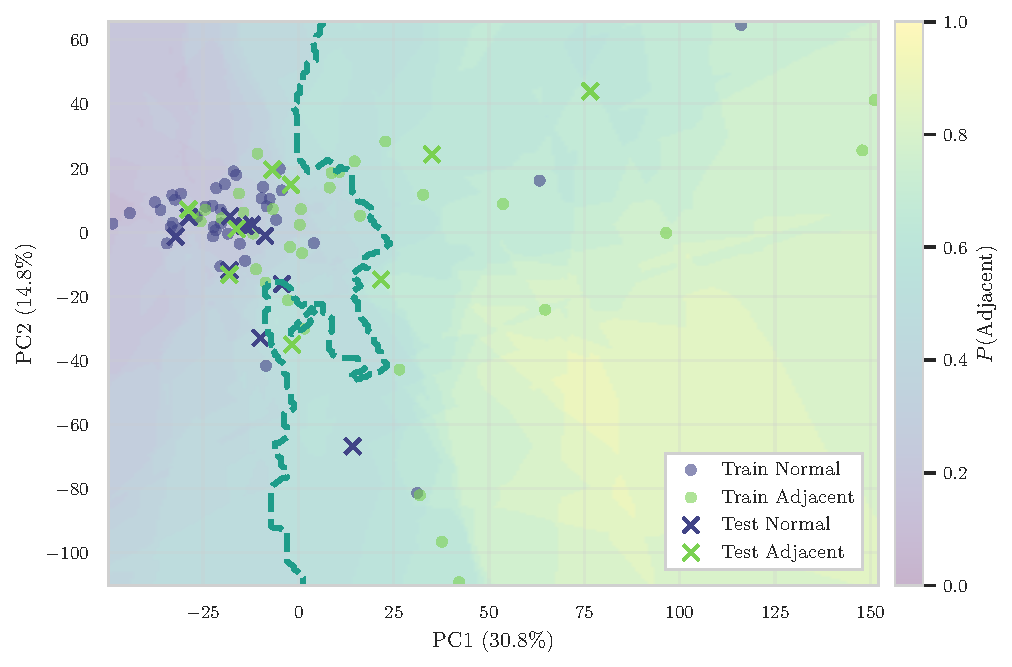
\includegraphics[width=0.5\linewidth]{images/cap6/GSE69914_knn_boundary.pdf}
    \caption{Projection of the KNN decision surface onto PC1--PC2
           (explaining 30.8\% and 14.8\% of variance, respectively).
           Train and test samples from both classes overlap extensively,
           with no geometrically separable structure.}
    \label{fig:gse69914_boundary}
\end{figure}

\paragraph{Compression to 50 CpGs via MILP}

\begin{table}[t]
\centering
\scriptsize
\caption{Performance metrics --- KNN, 50 CpGs (GSE69914, internal test).}
\label{tab:gse69914_50}
\begin{tabular}{c c c c c c}
\toprule
AUC & BAcc & Precision & Recall & F1-score & MCC \\
\midrule
0.6500 & 0.6167 & 0.7500 & 0.3333 & 0.4615 & 0.2858 \\
\bottomrule
\end{tabular}
\end{table}

\begin{figure}[t]
\centering
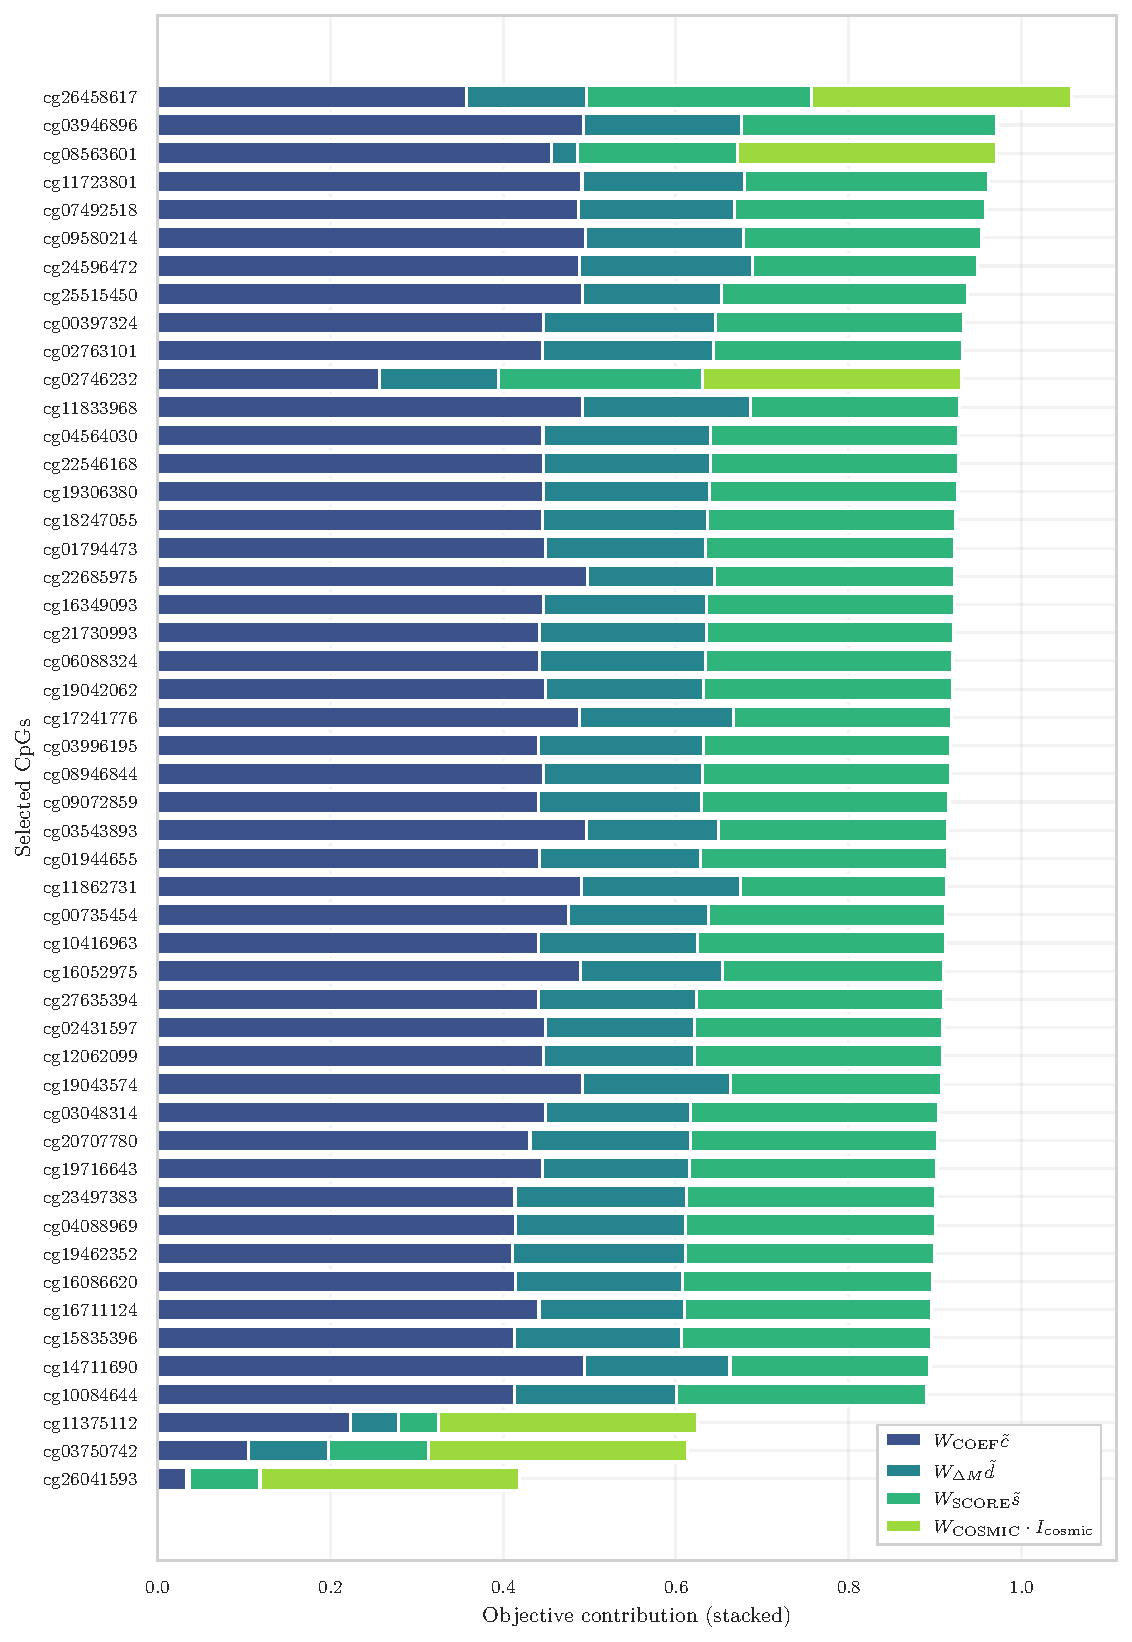
\includegraphics[width=0.75\textwidth]
  {images/cap6/GSE69914_knapsack_selected_contributions_stacked.pdf}
\caption{Component-wise decomposition of the MILP objective for the 50-CpG
panel in GSE69914. Each bar is one selected locus, sorted by total utility;
stacked segments show contributions from
$w_{\mathrm{coef}}\tilde{c}$,
$w_{\Delta M}\tilde{d}$,
$w_{\sigma}\tilde{s}$, and
$w_{\mathrm{COSMIC}} \cdot \mathbf{1}_{\mathrm{cosmic}}$.}
\label{fig:gse69914_compression}
\end{figure}

Following the intra-dataset KNN training, the learned permutation importance
scores --- alongside the absolute $\Delta M$ effect sizes and the inverse
baseline variability scores --- are fed as input to the MILP formulation of
Section~\ref{sec:knapsack}. The resulting 50-CpG panel, selected under
$\mu = 1.0$ and $w_{\mathrm{COSMIC}} = 1$, is shown in
Figure~\ref{fig:gse69914_compression} with its component-wise utility
decomposition. A KNN classifier retrained exclusively on these 50 loci yields
the metrics in Table~\ref{tab:gse69914_50}. Threshold-level metrics are identical to the 5,000-CpG model, indicating that
the compressed panel reproduces the same decision structure at 100-fold lower
dimensionality. The AUC reduction ($0.78 \to 0.65$) reflects the loss of loci
with marginal discriminative weight that contributed to the ranking surface but
not to the operating threshold. The score distributions
(Figure~\ref{fig:gse69914_scores}) confirm that neither panel version achieves
confident class separation, while the decision boundary and importance--effect
analysis (Figure~\ref{fig:gse69914_boundary}) show a weak Spearman correlation
($\rho = -0.22$) between classifier importance and $|\Delta M|$, indicating
that discriminative and biologically drifted loci are not well aligned in this
cohort.

\begin{figure}[t]
\centering
\begin{subfigure}[b]{0.48\textwidth}
  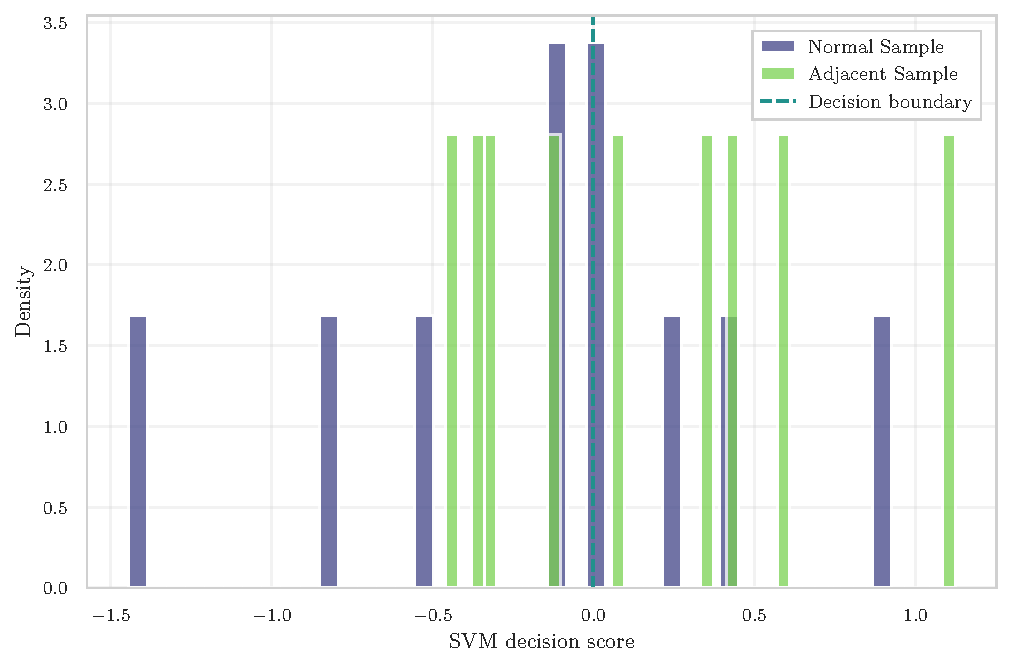
\includegraphics[width=\textwidth]
    {images/cap6/GSE69914_ScoreDist.pdf}
  \caption{Predicted probability distribution for the 50000-CpG panel.}
\end{subfigure}
\hfill
\begin{subfigure}[b]{0.48\textwidth}
  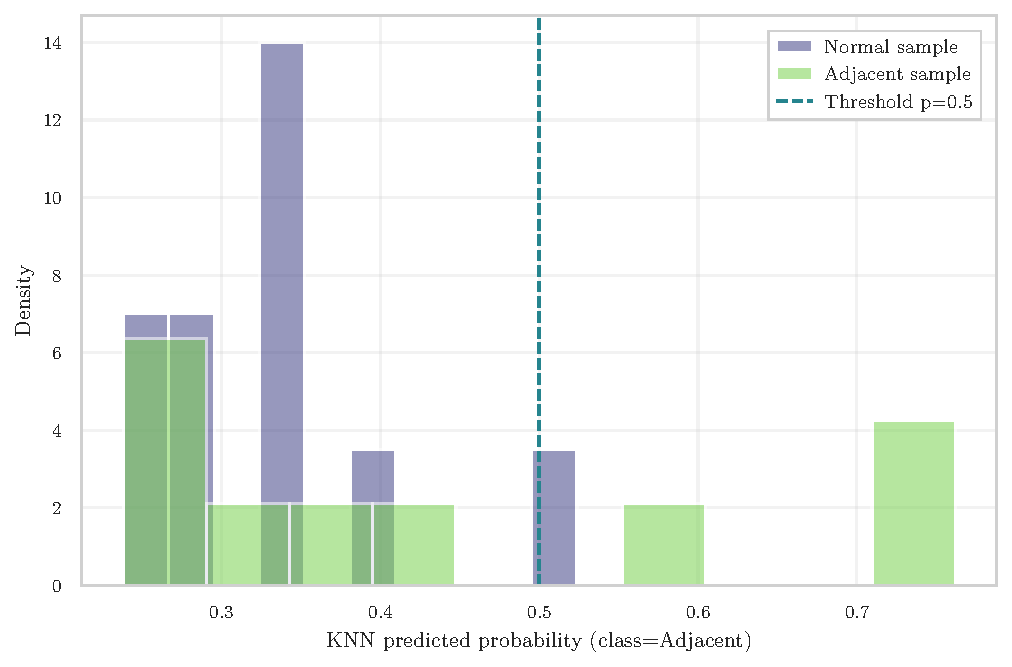
\includegraphics[width=\textwidth]
    {images/cap6/GSE69914_knncheck_proba_dist_50cpg.pdf}
  \caption{Predicted probability distribution for the 50-CpG panel.}
\end{subfigure}
\caption{Score distributions for Normal and Adjacent samples in GSE69914.}
\label{fig:gse69914_scores}
\end{figure}

\paragraph{Separation along the Tumor axis}

To verify that the Normal--Adjacent--Tumor biological axis is preserved in the
feature space, the same KNN classifier trained to discriminate Normal from
Adjacent tissue is evaluated on a Normal~(test split) versus Tumor~(all
available samples) comparison, without any retraining. This zero-shot
evaluation yields AUC = 1.000 and mean $|\Delta M| = 1.84$, confirming that
the dataset harbours a strong tumour-driven methylation signal that projects
clearly onto the learned discriminative axis. The comparatively subtle
performance on the Normal--Adjacent task therefore reflects the biological
attenuation of the field-cancerization signal rather than a failure of the
feature space, consistent with the model of progressive epigenetic drift
discussed in Chapter~\ref{chap:biological_background}.



\paragraph{Gene-level coherence and functional enrichment}

The 50-CpG panel maps to 40 unique genes. The component-wise decomposition
of the MILP objective (Figure~\ref{fig:gse69914_compression}) shows that most
selected loci carry contributions from all three statistical components
($w_{\mathrm{coef}}\tilde{c}$, $w_{\Delta M}\tilde{d}$,
$w_{\sigma}\tilde{s}$), with a subset receiving additional weight from the
COSMIC indicator. Among the COSMIC-annotated loci, four genes warrant
biological commentary.

\textbf{BRCA2} (cg26458617, hypomethylated in Adjacent): a tumour suppressor
central to homologous recombination repair of double-strand DNA breaks;
germline mutations substantially increase lifetime risk of breast and ovarian
cancer, and promoter methylation of \textit{BRCA2} has been linked to the
BRCAness phenotype in sporadic tumours, potentially conferring sensitivity to
PARP inhibitor therapy~\cite{kalachand2024brca}.

\textbf{BARD1} (cg08563601, hypermethylated in Adjacent): the obligate
heterodimeric partner of BRCA1 in the RING-domain complex involved in DNA
repair and apoptosis; loss-of-function variants in \textit{BARD1} confer a
moderate penetrance risk for breast cancer (OR $\approx$ 2.90), with
particularly elevated risk in triple-negative breast cancer~\cite{graffeo2022bard1}.

\textbf{MAP2K4} (cg02746232, hypermethylated in Adjacent): a MAPKK-family
kinase that activates both the JNK and p38 stress-response axes; its role in
breast cancer is context-dependent, with homozygous deletions and loss-of-function
mutations identified in breast carcinomas supporting a tumour-suppressive function,
while overexpression has also been reported to promote invasion via PI3K/AKT
activation~\cite{su1998mkk4,liu2019map2k4}.

\textbf{RBPJ} (cg22002629, hypermethylated in Adjacent): the canonical
transcriptional effector of the Notch signalling pathway, acting as a
context-dependent repressor or activator of target gene expression; Notch--RBPJ
dysregulation contributes to breast cancer progression, cancer stem cell
maintenance, and resistance to therapy~\cite{stylianou2021notch}.


GO Biological Process analysis identifies focussed enrichment in DNA damage
surveillance and chromatin ubiquitination (Table~\ref{tab:gse69914_go}),
consistent with the BRCA2--BARD1 axis present in the panel.
\paragraph{Cross-dataset transferability}

External evaluation yields near-random discrimination on both target cohorts:
AUC = 0.517 on GSE225845 and AUC = 0.498 on GSE287331, with balanced
accuracy collapsing to 0.5 and zero recall for the Adjacent class in both
cases. The failure is symmetric across targets, ruling out a directional
mismatch specific to one partner cohort and suggesting instead that the
discriminative direction identified in GSE69914 does not project onto a
shared epigenetic axis --- a finding consistent with the low pairwise
$\Delta\beta$ concordance documented in Chapter~\ref{chap:feature_selection}.


\begin{figure}[t]
    \centering
    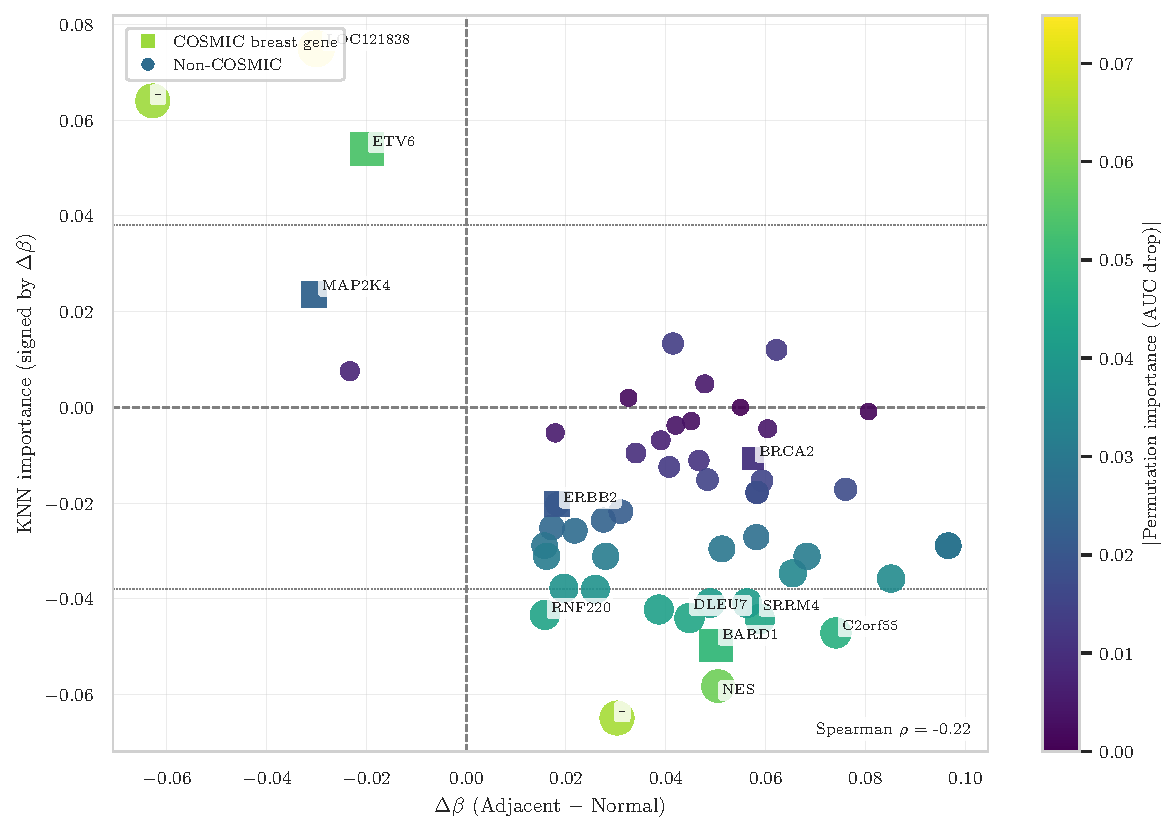
\includegraphics[width=0.5\linewidth]{images/cap6/GSE69914_volcano_50cpg.pdf}
    \caption{KNN permutation importance versus $\Delta M$ effect size
           (Adjacent $-$ Normal) for each of the 50 selected loci.
           COSMIC breast cancer genes are highlighted in green.
           The weak negative Spearman correlation ($\rho = -0.22$)
           indicates limited alignment between discriminative weight
           and biological effect size.}
    \label{ffig:gse69914_volcano}
\end{figure}


%-----------------------------------------------------------
\subsection{Dataset GSE225845}
\label{sec:results_gse225845}
%-----------------------------------------------------------

GSE225845 presents the clearest example of linear
separability in this study. The 5,000-CpG panel supports a
well-defined decision boundary with high AUC and balanced
class discrimination, and the 50-CpG compressed panel largely
preserves this structure. The cohort also provides an
informative reference point for the relationship between
field-cancerization and full tumour transformation: the same
compressed panel that discriminates Normal from Adjacent
tissue achieves even stronger separation against Tumor
samples, suggesting that the selected loci lie on the
biological continuum of progressive epigenetic drift rather
than encoding a tissue-contrast artefact.

\paragraph{Linear separability of the 5,000-CpG panel}

The linear SVM is evaluated under a stratified 80/20 split
($n_{\mathrm{train}} = 202$, $n_{\mathrm{test}} = 51$).
Performance is summarised in Table~\ref{tab:gse225845_5k}.

\begin{table}[H]
\centering
\caption{Performance metrics — Linear SVM, 5,000 CpGs
         (GSE225845, internal test)}
\label{tab:gse225845_5k}
\begin{tabular}{lc}
\toprule
Metric & Value \\
\midrule
AUC               & 0.9565 \\
PR-AUC            & 0.9623 \\
Balanced Accuracy & 0.9030 \\
Precision         & 0.9259 \\
Recall            & 0.8929 \\
F1-score          & 0.9091 \\
Specificity       & 0.9130 \\
MCC               & 0.8034 \\
\bottomrule
\end{tabular}
\end{table}

The confusion matrix
$\bigl[\begin{smallmatrix}21&2\\3&25\end{smallmatrix}\bigr]$
confirms balanced discrimination across classes. The high
MCC (0.80) rules out class-imbalance artefacts as a driver
of AUC inflation and indicates that the structurally
constrained 5,000-CpG panel retains substantial discriminative
signal within this cohort.

Figure~\ref{fig:gse225845_boundary} shows the calibrated
decision boundary projected onto the first two principal
components (PC1 = 29.6\%, PC2 = 10.9\% variance explained):
a clear inter-class separation is visible, with residual
overlap confined to the margin region.
Figure~\ref{fig:gse225845_scores} reports the SVM decision
score distributions for the 5,000-CpG and 50-CpG models
side by side; in both cases the class densities are well
separated around the decision threshold $f(x) = 0$.

\begin{figure}[H]
\centering
\begin{subfigure}[b]{0.48\textwidth}
  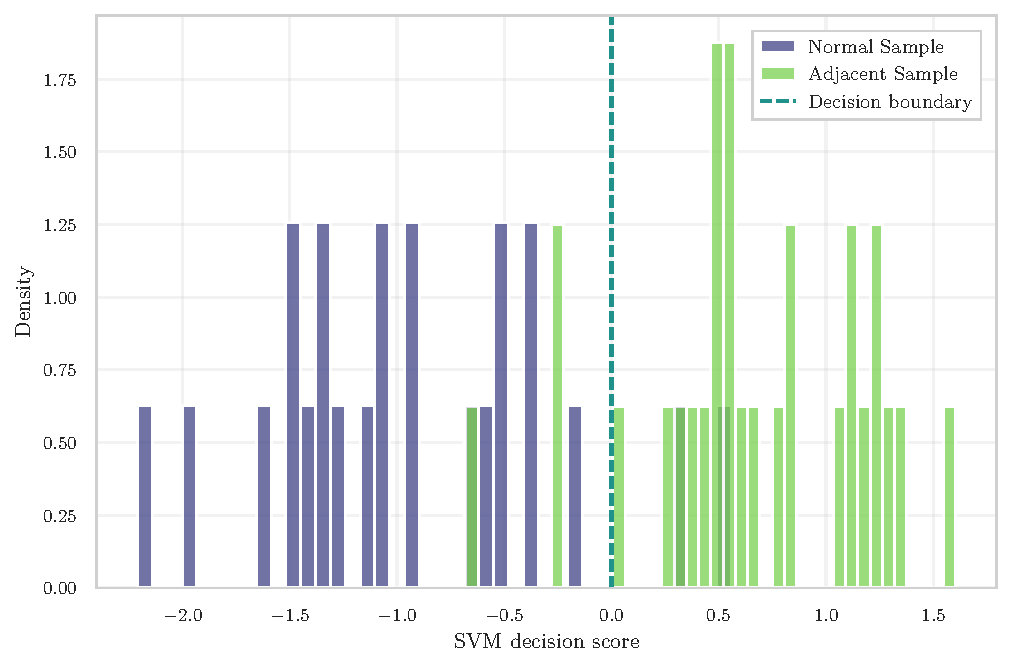
\includegraphics[width=\textwidth]
    {images/cap6/GSE225845_ScoreDist.pdf}
  \caption{Distribution of SVM decision scores
           for the 5,000-CpG panel.}
\end{subfigure}
\hfill
\begin{subfigure}[b]{0.48\textwidth}
  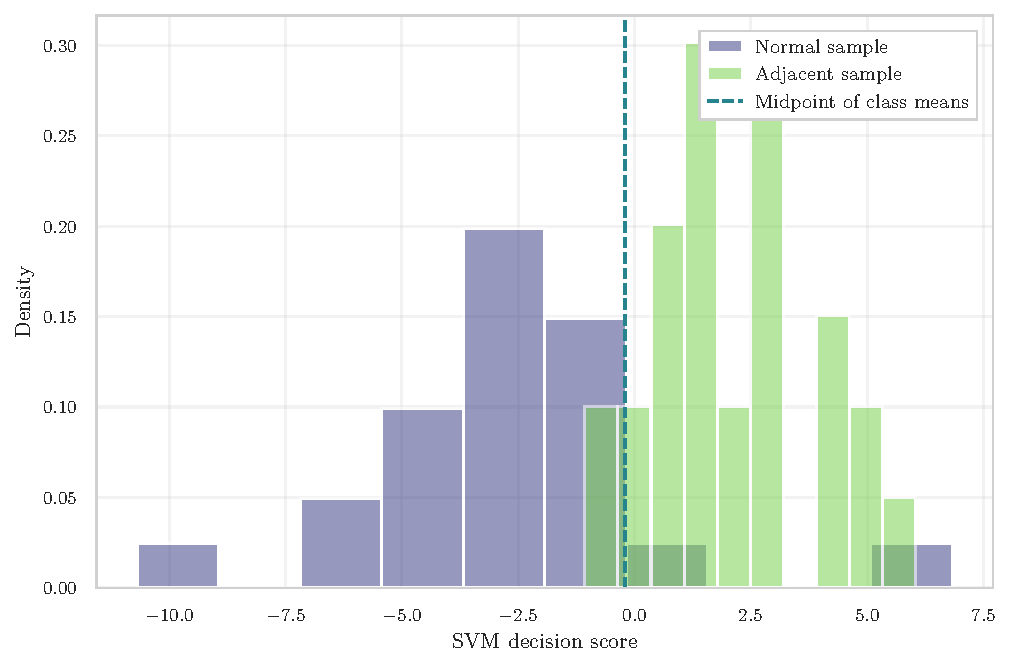
\includegraphics[width=\textwidth]
    {images/cap6/GSE225845_svmcheck_score_dist_50cpg.pdf}
  \caption{Distribution of SVM decision scores
           for the 50-CpG constrained panel.}
\end{subfigure}
\caption{
Score distributions for Normal and Adjacent samples under
the full 5,000-CpG panel and the
compressed 50-CpG subset in GSE225845.
}
\label{fig:gse225845_scores}
\end{figure}

\paragraph{Cross-dataset transferability of the
5,000-CpG panel}

Transferability is evaluated under the train-on-GSE225845 /
test-on-external paradigm of
Section~\ref{sec:cross_dataset}, restricting features to the
CpG intersection with each target cohort. On GSE69914
(2,893 intersecting CpGs), external performance degrades to
AUC = 0.578, with balanced accuracy = 0.5 and zero positive
predictions. On GSE287331 (3,970 intersecting CpGs),
performance collapses to AUC = 0.029, again with balanced
accuracy = 0.5 and no positive classifications. The
systematic failure across both targets, despite strong
internal discrimination, points to structural misalignment
of the inferred separating hyperplane with the epigenetic
drift orientation of the external cohorts. Crucially, the
collapse cannot be attributed to overfitting: internal
test performance under feature intersection remains stable
at AUC $\approx 0.92$.

\paragraph{Compression to 50 CpGs}

The constrained optimisation ($\mu = 0.5$,
$w_{\mathrm{COSMIC}} = 1$) yields the metrics in
Table~\ref{tab:gse225845_50}.

\begin{table}[H]
\centering
\caption{Performance metrics — Linear SVM, 50 CpGs
         (GSE225845, internal test)}
\label{tab:gse225845_50}
\begin{tabular}{lc}
\toprule
Metric & Value \\
\midrule
AUC               & 0.9363 \\
PR-AUC            & 0.8786 \\
Balanced Accuracy & 0.8851 \\
Precision         & 0.9231 \\
Recall            & 0.8571 \\
F1-score          & 0.8889 \\
Specificity       & 0.9130 \\
MCC               & 0.7666 \\
\bottomrule
\end{tabular}
\end{table}

The AUC decreases modestly ($0.9565 \to 0.9363$) while MCC
remains high (0.77). The confusion matrix
$\bigl[\begin{smallmatrix}21&2\\4&24\end{smallmatrix}\bigr]$
shows only one additional false negative relative to the
5,000-CpG model, confirming that a substantial fraction of
the discriminative structure is concentrated in a compact
subset of loci.

A positive Spearman correlation between signed SVM
coefficients and $\Delta\beta$ (Adjacent -- Normal,
$\rho = 0.38$) indicates partial concordance between
univariate effect size and multivariate discriminative
weight. Several loci display large coefficients despite
moderate $\Delta\beta$, suggesting that covariance
structure — rather than marginal shift alone — drives
discrimination. Figure~\ref{fig:gse225845_compression}
summarises the compressed panel diagnostics.

\begin{figure}[t]
\centering
\begin{subfigure}[b]{0.48\textwidth}
  
\includegraphics[width=\textwidth]
    {images/cap6/GSE225845_boundary_pca_prob_calibrated.pdf}
  \caption{Projection of the calibrated linear SVM decision surface
           onto the first two principal components (PC1$-$PC2).
           }
\end{subfigure}
\hfill
\begin{subfigure}[b]{0.48\textwidth}
  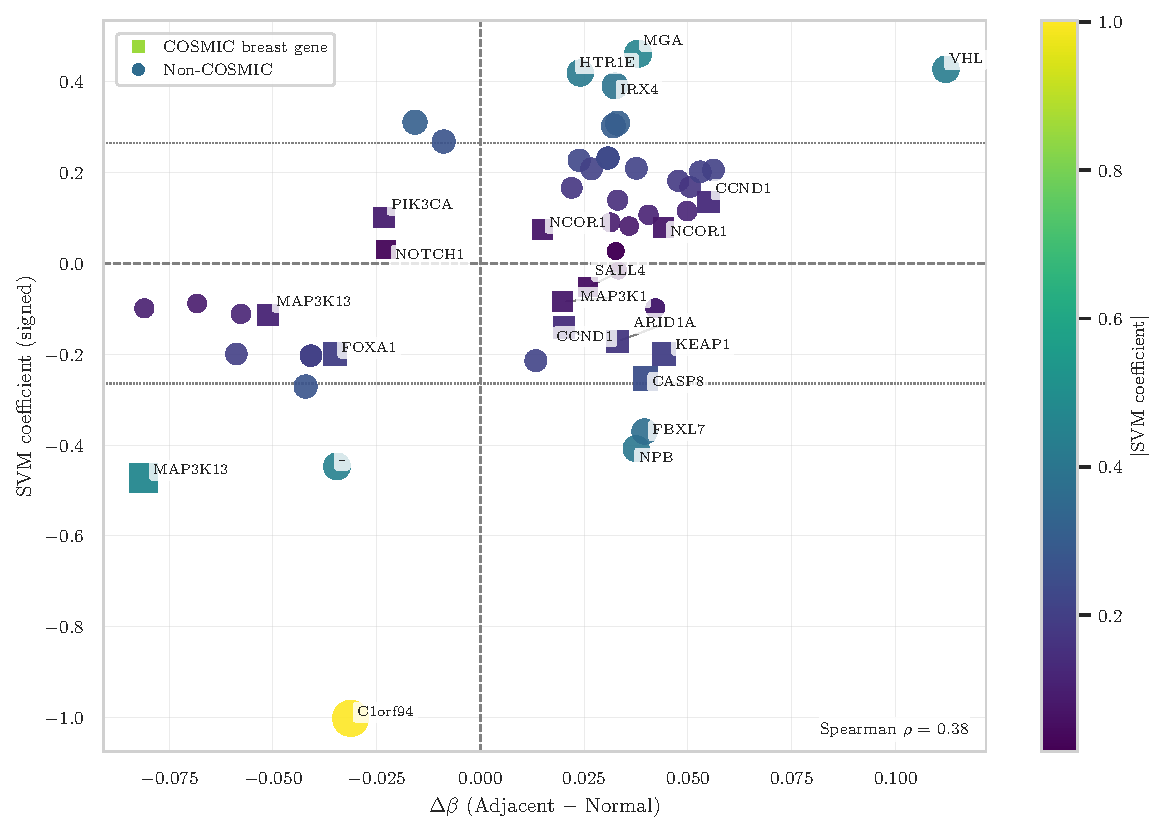
\includegraphics[width=\textwidth]
    {images/cap6/GSE225845_volcano_50cpg.pdf}
  \caption{Relationship between SVM coefficient magnitude and
           $\Delta M$ effect size (Adjacent $-$ Normal) for the
           constrained 50-CpG panel.}
\end{subfigure}
\caption{
Decision geometry and coefficient–effect-size relationship 
for the constrained 50-CpG predictive model in GSE225845. 
}  
\label{fig:gse225845_boundary} 
\end{figure}



\begin{figure}[t]
    \centering
    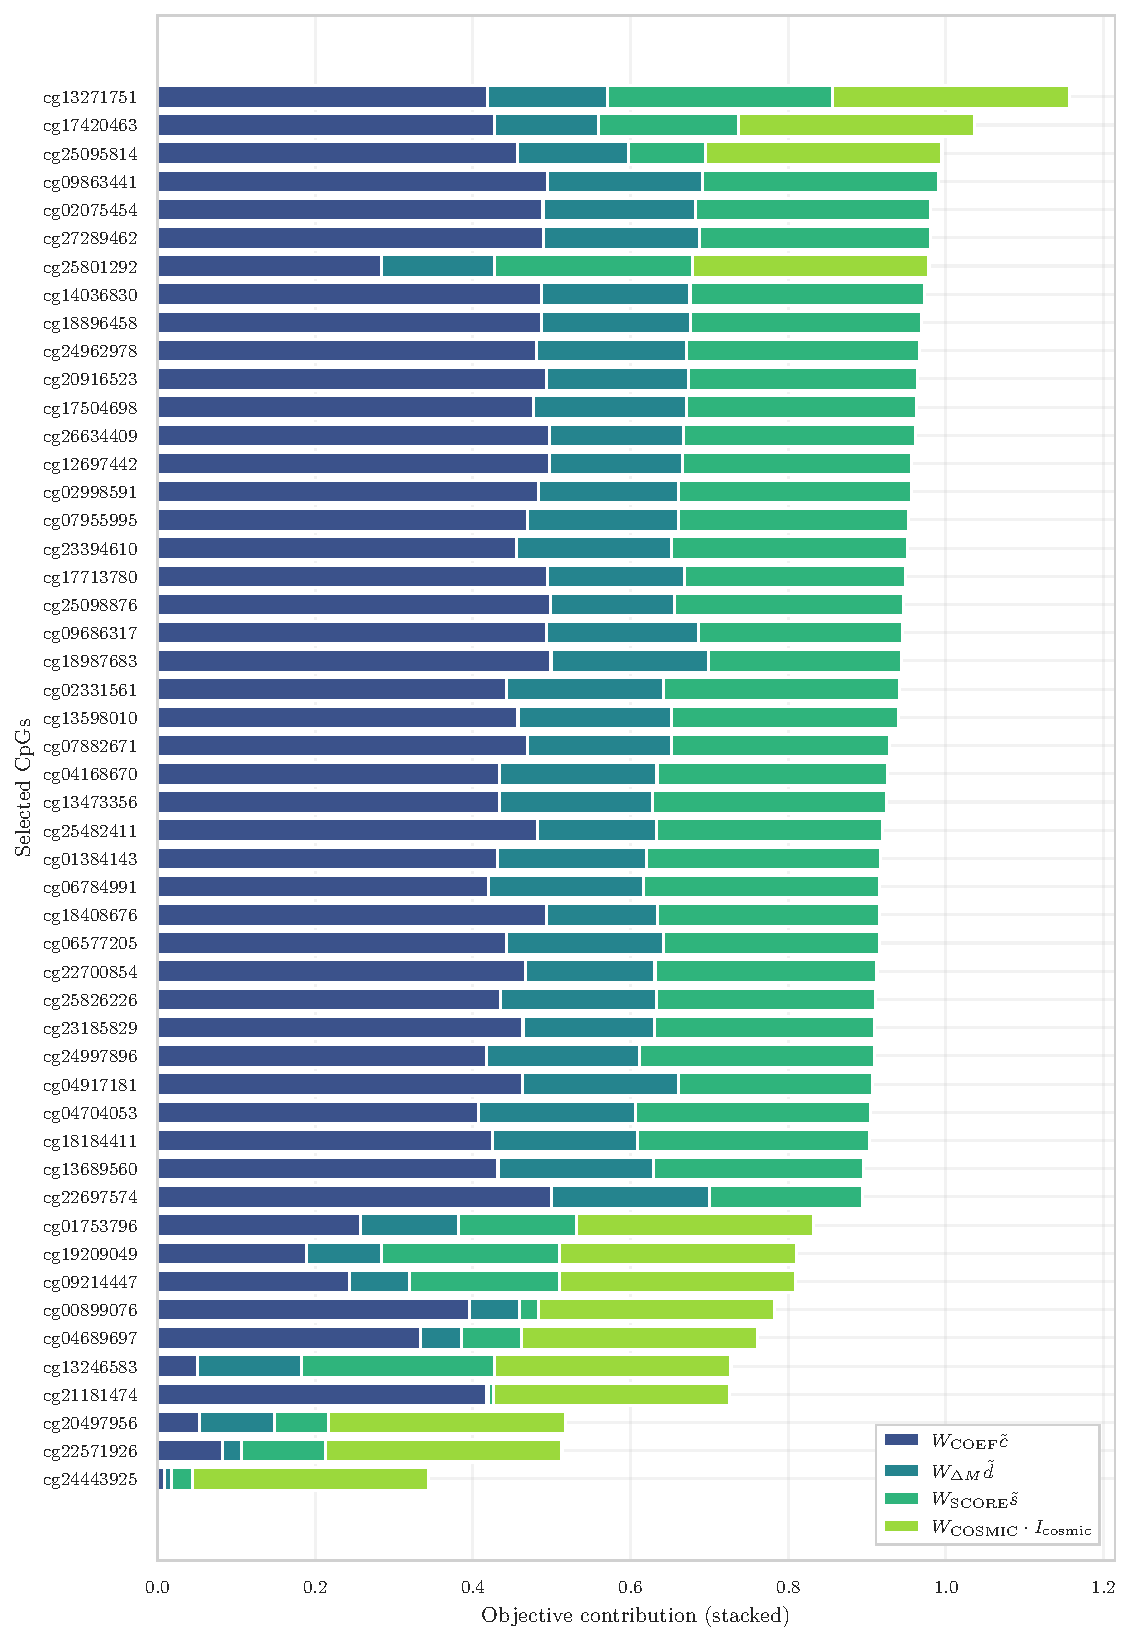
\includegraphics[width=0.75\textwidth]
    {images/cap6/GSE225845_knapsack_selected_contributions_stacked.pdf}
    \caption{ Component-wise decomposition of the MILP objective for the
selected 50-CpG panel in GSE225845.
    }
    \label{fig:gse225845_compression}
\end{figure}

An important observation concerns the behaviour of the
compressed panel beyond the Normal--Adjacent contrast for
which it was optimised. Evaluated on the Normal--Tumor
axis within the same cohort, the 50-CpG model achieves
AUC = $0.9118 \pm 0.0630$ (five-fold CV) with mean
$|\Delta M| = 0.955$, compared to AUC = $0.8170 \pm 0.0605$
and mean $|\Delta M| = 0.690$ on the Normal--Adjacent
task. The silhouette coefficient rises from 0.09 to 0.13.
Rather than reflecting a conflation of the two contrasts,
this gradient is consistent with the biological model of
progressive epigenetic drift: the loci selected to
discriminate the subtle Normal--Adjacent transition lie
along the same methylation axis that becomes more
pronounced in full malignant transformation, and
their discriminative capacity scales accordingly.

\paragraph{Gene-level coherence and functional enrichment}

The 50-CpG compressed panel maps to 42 unique genes; of
the 50 loci, 44 are associated with COSMIC breast cancer
genes. No significant GO Biological Process terms are
identified at FDR $< 0.05$. KEGG analysis reveals
significant enrichment for canonical oncogenic pathways
(Table~\ref{tab:gse225845_kegg}).

\begin{table}[H]
\centering
\caption{KEGG enrichment — 50-CpG panel (GSE225845)}
\label{tab:gse225845_kegg}
\begin{tabular}{lcc}
\toprule
Pathway & Overlap & Adj.\ $p$ \\
\midrule
Thyroid hormone signaling pathway & 4/121 & 0.0165 \\
Hepatocellular carcinoma          & 4/168 & 0.0289 \\
Pathways in cancer                & 6/531 & 0.0365 \\
\bottomrule
\end{tabular}
\end{table}

The enrichment is driven by \textit{NCOR1}, \textit{NOTCH1},
\textit{PIK3CA}, \textit{CCND1}, \textit{KEAP1},
\textit{ARID1A}, \textit{CASP8}, and \textit{VHL} — a set
that spans PI3K/AKT signalling, cell-cycle control, chromatin
remodelling, and apoptosis regulation, all recurrently
implicated in breast tumorigenesis. MSigDB Hallmark analysis
further identifies \textit{Notch Signaling} (2/32 genes,
FDR = 0.033), driven by \textit{NOTCH1} and \textit{CCND1}.
The convergence of two independent pathway collections on
Notch and canonical oncogenic modules strengthens the
evidence for biological coherence of the compressed panel.
Taken together, GSE225845 exhibits strong intra-cohort linear
separability, robust signal retention under compression, and
convergence of the optimised panel toward established cancer
signalling networks. The failure of cross-dataset transfer,
however, confirms that the learned separating axis is
cohort-specific and does not generalise across independent
methylation landscapes.

%-----------------------------------------------------------
\subsection{Dataset GSE287331}
\label{sec:results_gse287331}
%-----------------------------------------------------------

GSE287331 occupies the opposite end of the separability
spectrum relative to GSE69914. The Normal--Adjacent contrast
is characterised by a large mean $|\Delta M|$ and a high
silhouette coefficient, yielding perfect internal
classification at both 5,000 and 50 CpGs. At the same time,
cross-dataset transfer fails completely, confirming that the
discriminative axis learned in this cohort is structurally
inverted relative to the shared drift orientation of the
other two datasets — a property already anticipated by the
inter-dataset stability analysis of
Chapter~\ref{chap:feature_selection}.

\paragraph{Linear separability of the 5,000-CpG panel}

The linear SVM achieves perfect separation on the internal
test set ($n_{\mathrm{test}} = 49$: 37 Normal, 12 Adjacent).
Performance metrics are reported in
Table~\ref{tab:gse287331_5k}.

\begin{table}[H]
\centering
\caption{Performance metrics — Linear SVM, 5,000 CpGs
         (GSE287331, internal test)}
\label{tab:gse287331_5k}
\begin{tabular}{lc}
\toprule
Metric & Value \\
\midrule
AUC               & 1.0000 \\
Balanced Accuracy & 1.0000 \\
Precision         & 1.0000 \\
Recall            & 1.0000 \\
F1-score          & 1.0000 \\
Specificity       & 1.0000 \\
MCC               & 1.0000 \\
\bottomrule
\end{tabular}
\end{table}

The confusion matrix shows zero misclassifications across
both classes. The PCA projection confirms a two-cluster
geometry with a wide, uncontested margin and no borderline
samples. Perfect internal performance in this context is
not indicative of overfitting: the silhouette coefficient
of 0.40 and mean $|\Delta M| = 2.40$ on the test set
document a genuinely large effect size, and the signal is
structurally concentrated enough that even 50 CpGs suffice
to encode it completely (see below).

\paragraph{Compression to 50 CpGs}

The constrained optimisation ($\mu = 1.0$,
$w_{\mathrm{COSMIC}} = 0.7$) preserves complete
separability, as reported in Table~\ref{tab:gse287331_50}.

\begin{table}[H]
\centering
\caption{Performance metrics — Linear SVM, 50 CpGs
         (GSE287331, internal test)}
\label{tab:gse287331_50}
\begin{tabular}{lc}
\toprule
Metric & Value \\
\midrule
AUC               & 1.0000 \\
Balanced Accuracy & 1.0000 \\
Precision         & 1.0000 \\
Recall            & 1.0000 \\
F1-score          & 1.0000 \\
Specificity       & 1.0000 \\
MCC               & 1.0000 \\
\bottomrule
\end{tabular}
\end{table}

The equivalence between 5,000 and 50 CpGs demonstrates
that the discriminative signal is intrinsically
low-dimensional: a single compact subset of loci is
sufficient to encode the separating axis without any
loss of margin. Figure~\ref{fig:gse287331_scores}
shows the decision score distributions for both panel
sizes; complete class separation with no density overlap
is visible in both panels.

\begin{figure}[t]
\centering
\begin{subfigure}[b]{0.48\textwidth}
  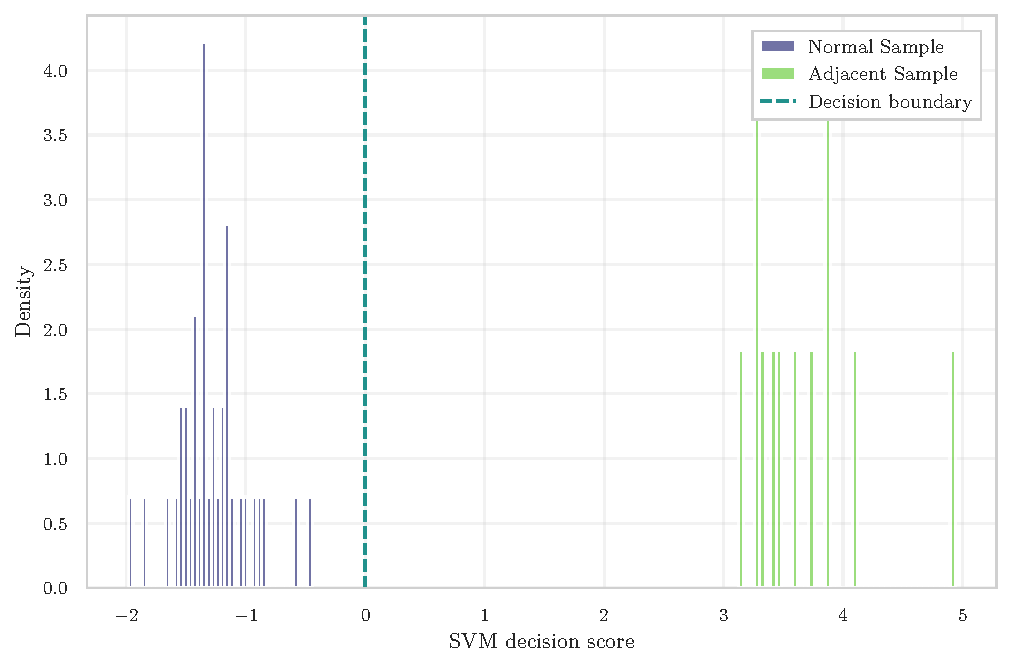
\includegraphics[width=\textwidth]
    {images/cap6/GSE287331_ScoreDist.pdf}
  \caption{Distribution of SVM decision scores
           for the 5,000-CpG panel.}
\end{subfigure}
\hfill
\begin{subfigure}[b]{0.48\textwidth}
  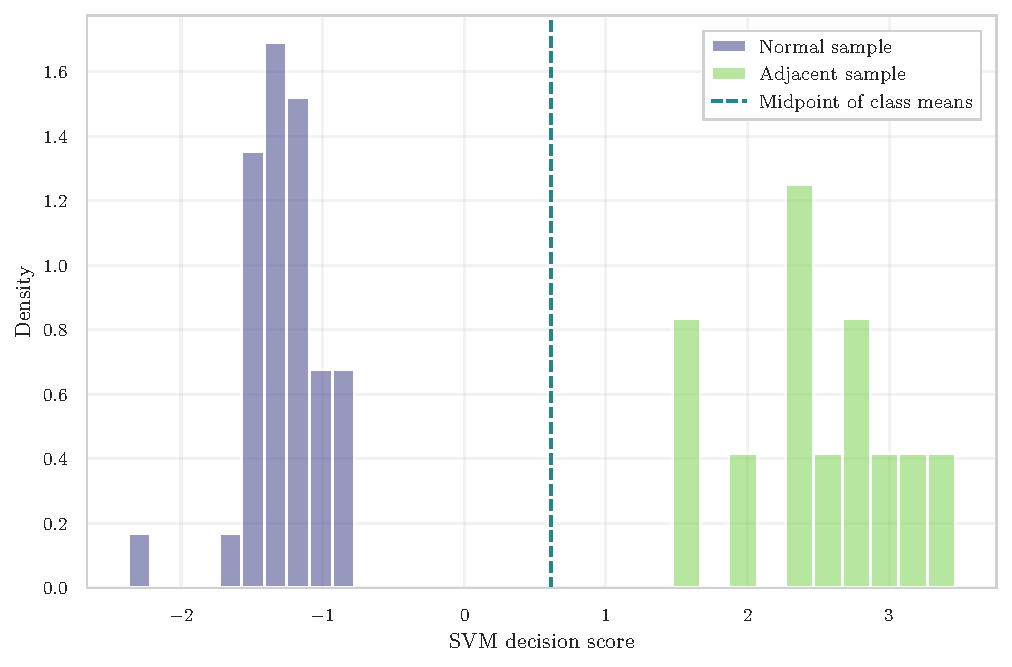
\includegraphics[width=\textwidth]
    {images/cap6/GSE287331_svmcheck_score_dist_50cpg.pdf}
  \caption{Distribution of SVM decision scores
           for the 50-CpG constrained panel.}
\end{subfigure}
\caption{
Score distributions for Normal and Adjacent samples under
the full 5,000-CpG panel and the
compressed 50-CpG subset in GSE287331.
}
\label{fig:gse287331_scores}
\end{figure}

\begin{figure}[t]
\centering
\begin{subfigure}[b]{0.48\textwidth}
  
\includegraphics[width=\textwidth]
    {images/cap6/GSE287331_boundary_pca_prob_calibrated.pdf}
  \caption{Projection of the calibrated linear SVM decision surface
           onto the first two principal components (PC1$-$PC2).
           }
\end{subfigure}
\hfill
\begin{subfigure}[b]{0.48\textwidth}
  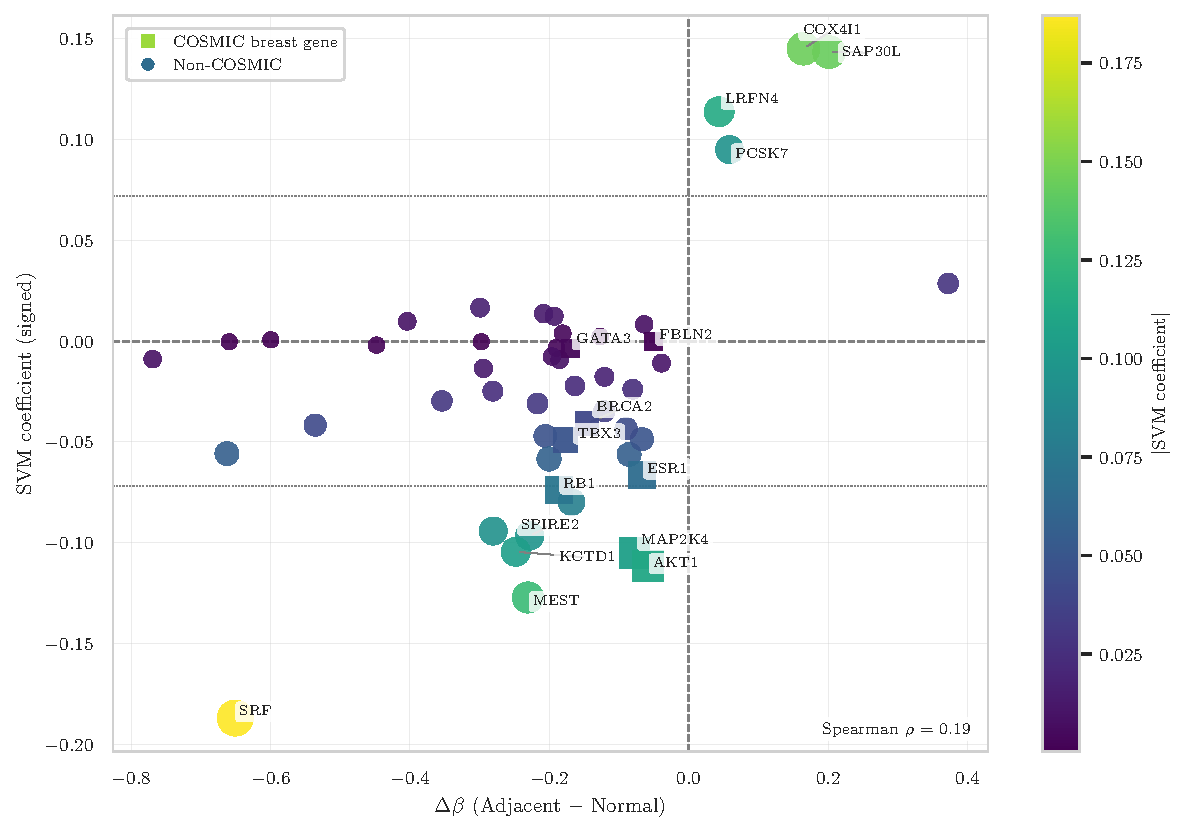
\includegraphics[width=\textwidth]
    {images/cap6/GSE287331_volcano_50cpg.pdf}
  \caption{Relationship between SVM coefficient magnitude and
           $\Delta M$ effect size (Adjacent $-$ Normal) for the
           constrained 50-CpG panel.}
\end{subfigure}
\caption{
Decision geometry and coefficient–effect-size relationship 
for the constrained 50-CpG predictive model in GSE287331. 
}  
\label{fig:gse287331_boundary} 
\end{figure}



As with GSE225845, the compressed panel generalises
naturally to the Normal--Tumor contrast. Evaluated on
Normal versus Tumor tissue within the same cohort
($n = 106$: 37 Normal, 69 Tumor), the 50-CpG model
achieves AUC = 1.000 ($\pm 0.000$, five-fold CV),
silhouette = 0.44, and mean $|\Delta M| = 1.98$ —
marginally below the Normal--Adjacent values
(silhouette = 0.40, mean $|\Delta M| = 2.40$). This
reversal of the usual ordering, in which Adjacent tissue
is harder to distinguish from Normal than Tumor is,
reflects the structural peculiarity of GSE287331:
the Normal--Adjacent drift in this cohort is not merely
detectable but exceptionally strong, exceeding the
Normal--Tumor methylation distance along the principal
component axis (PC1 projection 0.48 vs.\ 0.40). The
implication is that the 50 selected loci are particularly
sensitive to the early field-defect rather than to the
full malignant transition, a property that further
distinguishes this cohort from the shared drift axis
of GSE69914 and GSE225845.

Figure~\ref{fig:gse287331_compression} reports the
compressed panel diagnostics.


\begin{figure}[t]
    \centering
    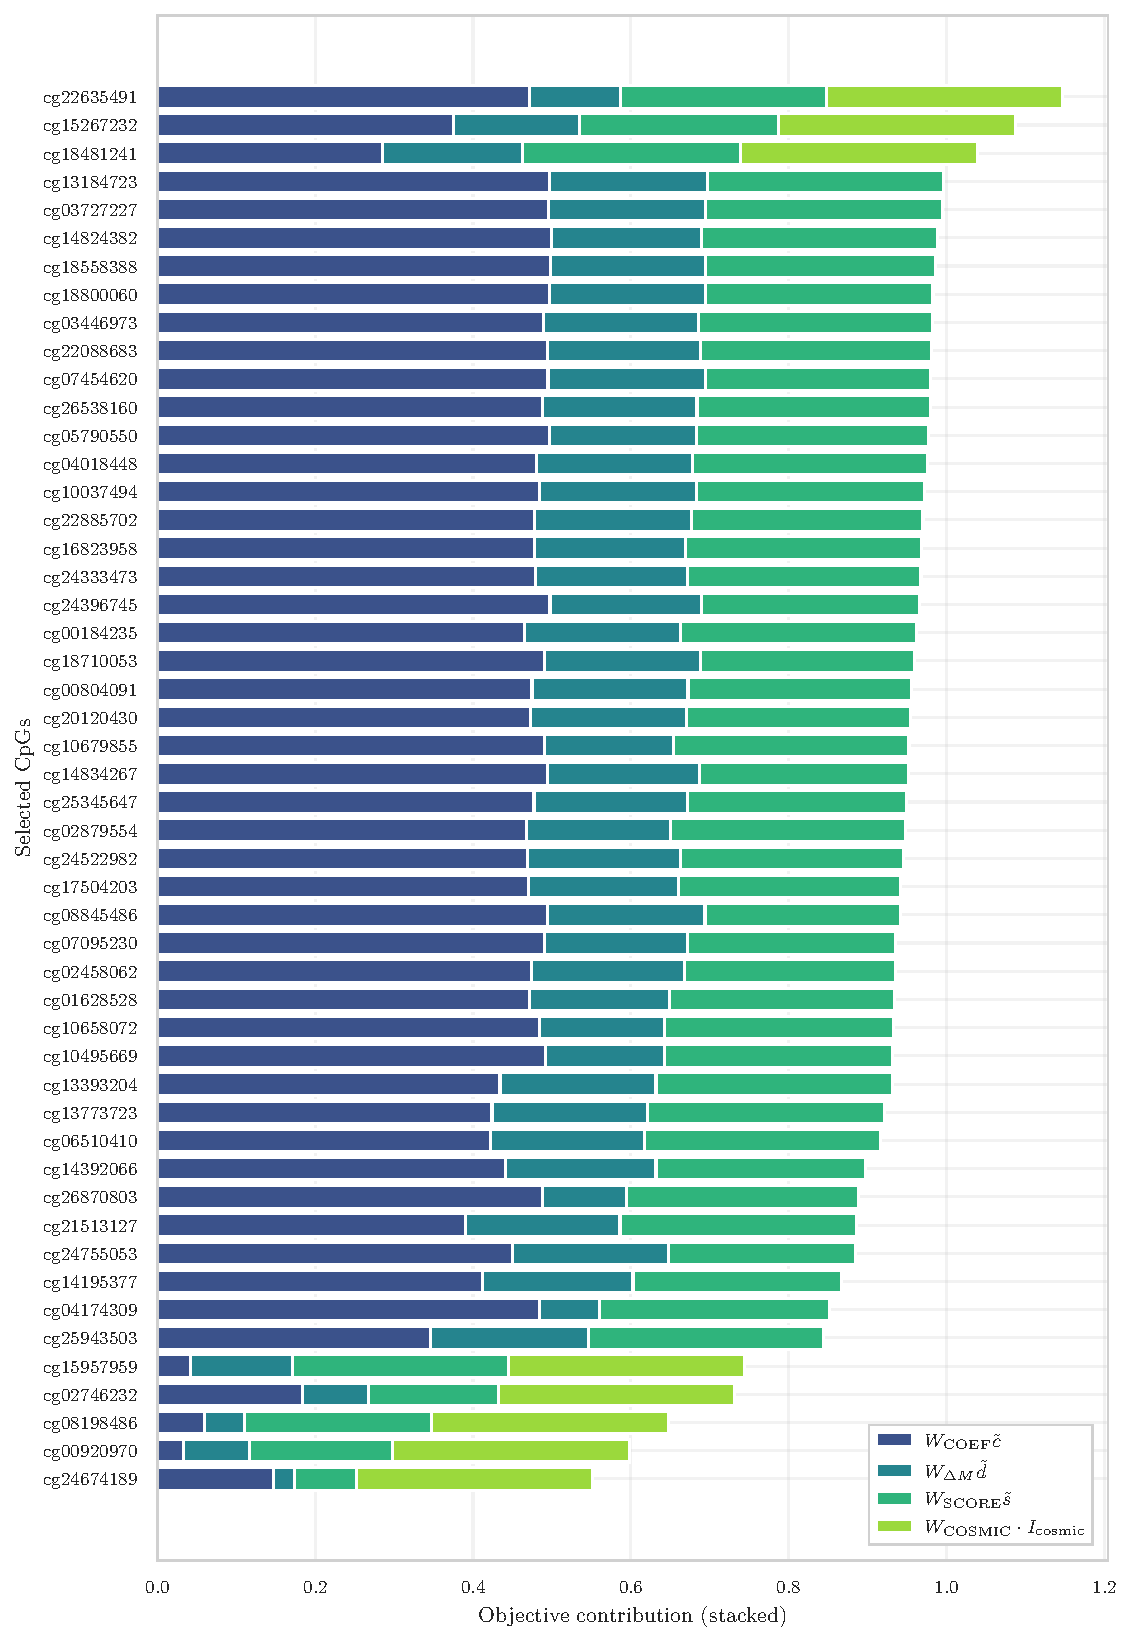
\includegraphics[width=0.75\textwidth]
    {images/cap6/GSE287331_knapsack_selected_contributions_stacked.pdf}
    \caption{ Component-wise decomposition of the MILP objective for the
selected 50-CpG panel in GSE287331.
    }
    \label{fig:gse287331_compression}
\end{figure}

\paragraph{Cross-dataset transferability}

Despite perfect internal classification, external
evaluation reveals complete loss of discriminative
ability: AUC = 0.436 on GSE69914 and AUC = 0.510 on
GSE225845, with balanced accuracy collapsing to 0.5
and zero recall for the Adjacent class in both cases.
Notably, performance on GSE69914 falls below random
expectation (AUC $< 0.5$), consistent with directional
inversion of the learned separating hyperplane rather
than mere signal absence. This pattern confirms that
GSE287331 encodes a distinct epigenetic regime whose
drift orientation is systematically anti-correlated with
the shared axis of the other two cohorts, as established
in Chapter~\ref{chap:feature_selection}. The dichotomy
between perfect internal separability and zero external
transfer is therefore not paradoxical: it reflects the
coexistence of a strong but cohort-specific methylation
signal with a structural misalignment that prevents
cross-cohort generalisation.

\paragraph{Gene-level coherence and functional enrichment}

The 50-CpG panel maps to 42 unique genes. Unlike
GSE225845, GO Biological Process analysis identifies
significant enrichment terms
(Table~\ref{tab:gse287331_go}), while KEGG analysis
converges on core oncogenic pathways
(Table~\ref{tab:gse287331_kegg}).

\begin{table}[H]
\centering
\caption{GO Biological Process enrichment — 50-CpG panel
         (GSE287331)}
\label{tab:gse287331_go}
\begin{tabular}{lcc}
\toprule
Term & Overlap & Adj.\ $p$ \\
\midrule
Response to lipid                      & 4/110 & 0.0429 \\
Regulation of protein kinase activity  & 4/119 & 0.0429 \\
Cellular response to TNF               & 4/119 & 0.0429 \\
\bottomrule
\end{tabular}
\end{table}

\begin{table}[H]
\centering
\caption{KEGG enrichment — 50-CpG panel (GSE287331)}
\label{tab:gse287331_kegg}
\begin{tabular}{lcc}
\toprule
Pathway & Overlap & Adj.\ $p$ \\
\midrule
Breast cancer              & 4/147 & 0.0477 \\
Pancreatic cancer          & 3/76  & 0.0477 \\
Small cell lung cancer     & 3/92  & 0.0477 \\
Epstein--Barr virus infection & 4/202 & 0.0477 \\
\bottomrule
\end{tabular}
\end{table}

The enrichment is driven by \textit{RB1}, \textit{AKT1},
\textit{BRCA2}, \textit{ESR1}, \textit{TRAF4},
\textit{MAP2K4}, and \textit{GATA3} — spanning PI3K/AKT
signalling, cell-cycle control, homologous recombination
repair, estrogen receptor signalling, and luminal lineage
determination, all well-established axes of breast cancer
biology. The GO terms further point toward inflammatory
signalling (TNF response) and lipid-mediated regulation,
extending the picture beyond canonical oncogenic modules.
The convergence of both KEGG and GO enrichment on
biologically plausible breast cancer processes confirms
that the compressed panel, despite being derived from a
cohort with inverted drift orientation, selects loci
embedded in functionally coherent genomic neighbourhoods.
The absence of cross-dataset transferability therefore
reflects a structural property of the methylation
landscape rather than a failure of the optimisation
to identify biologically meaningful loci.



%-----------------------------------------------------------
\section{Inter-Dataset Structure and Batch--Biology
         Diagnostics}
\label{sec:inter_dataset}
%-----------------------------------------------------------

The intra-dataset results of Section~\ref{sec:results_gse69914}--\ref{sec:results_gse287331}
establish that each cohort supports robust within-cohort
discrimination, but that no trained classifier transfers
successfully to an external dataset. Before concluding that
this failure is purely biological in origin, it is necessary
to quantify how much of the joint methylation variance is
attributable to dataset identity rather than to phenotype,
and whether the directional structure of the Normal--Adjacent
drift is preserved across cohorts or systematically distorted.
The diagnostics presented in this section address both
questions and directly motivate the representation-learning
strategy of Chapter~\ref{chap:multi_cohort_integration}.

%-----------------------------------------------------------
\subsection{PC1 as a Diagnostic Axis: Biological Signal
            versus Batch Structure}
\label{sec:pc1_diagnostic}
%-----------------------------------------------------------

The discriminative power of the first principal component
(PC1), computed on the union panel of all three cohorts,
is evaluated in two complementary settings: within-dataset
phenotype separation (Normal vs.\ Adjacent) and
between-dataset separation (cohort identity). The
juxtaposition of these two AUC values for the same axis
quantifies the relative dominance of biological versus
technical variance in the leading principal direction.

\paragraph{Within-dataset biological signal}

PC1 discriminates Normal from Adjacent tissue with AUC = 0.703
in GSE69914, AUC = 0.677 in GSE225845, and AUC = 1.000 in
GSE287331. Biological variation is therefore encoded in the
leading variance component across all three cohorts, most
strongly so in GSE287331, consistent with its intrinsically
large Normal--Adjacent effect size documented in
Section~\ref{sec:results_gse287331}.

\paragraph{Between-dataset batch effect}

When PC1 is used to discriminate cohort identity, the AUC
values are 0.806 (GSE69914 vs.\ GSE225845), 0.987 (GSE69914
vs.\ GSE287331), and 0.994 (GSE225845 vs.\ GSE287331). In
all three comparisons the batch-separation AUC meets or
exceeds the corresponding phenotype-separation AUC, and for
pairs involving GSE287331 the inter-dataset discrimination is
near-perfect. Figure~\ref{fig:batch_vs_biology} summarises
these values side by side.

\begin{figure}[H]
\centering
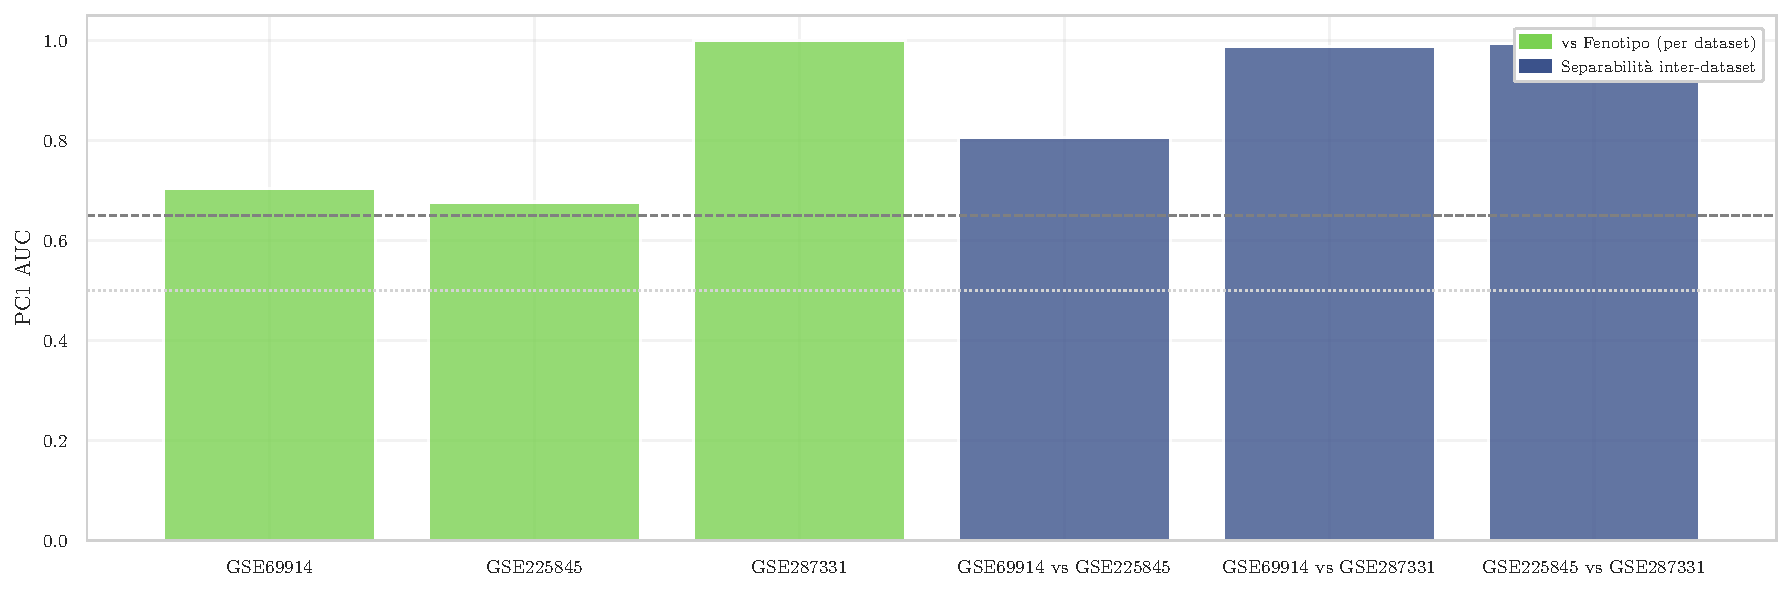
\includegraphics[width=0.65\textwidth]
  {images/cap6/6x5_batch_vs_biology_barplot}
\caption{PC1 discriminative power for phenotype separation
         (Normal vs.\ Adjacent, within each dataset) and for
         batch separation (between datasets), reported as AUC.
         In all pairwise comparisons, dataset identity is at
         least as separable as biological class.}
\label{fig:batch_vs_biology}
\end{figure}

These results confirm that, in the joint feature space,
dataset origin dominates the leading variance axis.
Any cross-cohort modelling strategy that operates directly
in this space will therefore capture batch structure before
biological signal, explaining the systematic collapse of
cross-dataset transfer performance documented in
Section~\ref{sec:cross_dataset}.

%-----------------------------------------------------------
\subsection{Directional Concordance of Methylation Shifts}
\label{sec:directional_concordance}
%-----------------------------------------------------------

A complementary diagnostic addresses the directional
structure of the Normal--Adjacent drift itself: even if
absolute effect sizes differ across cohorts, a shared
biological process would be expected to induce shifts of
consistent polarity at the same loci. Pairwise concordance
of $\Delta M$ (Adjacent -- Normal) is assessed via Spearman
correlation and sign agreement on the CpG intersection of
the three 5,000-CpG panels.

\paragraph{Pairwise concordance metrics}

\begin{table}[H]
\centering
\caption{Pairwise $\Delta M$ concordance across cohorts.}
\label{tab:pairwise_concordance}
\begin{tabular}{lcc}
\toprule
Pair & Spearman $\rho$ & Sign concordance \\
\midrule
GSE69914 vs.\ GSE225845  & 0.08 & 0.76 \\
GSE69914 vs.\ GSE287331  & 0.49 & 0.50 \\
GSE225845 vs.\ GSE287331 & 0.38 & 0.42 \\
\bottomrule
\end{tabular}
\end{table}

Two structurally distinct regimes emerge from
Table~\ref{tab:pairwise_concordance}. GSE69914 and
GSE225845 exhibit high sign concordance (76\%) with
near-zero rank correlation, indicating that the two cohorts
agree on the direction of the Normal--Adjacent shift at the
majority of shared loci but differ substantially in the
relative ordering of effect magnitudes. This pattern is
consistent with a shared biological axis whose expression
is modulated by platform-specific noise, cohort composition,
and effect-size scaling. Pairs involving GSE287331, by
contrast, show moderate rank correlation but sign
concordance at or below 50\%, indicating that the dominant
drift direction in GSE287331 is systematically inverted
relative to both partner cohorts — a structural inversion
rather than stochastic disagreement.

The scatter plots in Figure~\ref{fig:deltam_scatter}
visualise these patterns. In the GSE69914--GSE225845
comparison, points cluster symmetrically around the origin
with mild positive trend. In both comparisons involving
GSE287331, the point cloud is compressed toward the
vertical axis, reflecting the effect-size asymmetry, and
the sign inversion is apparent from the distribution of
points across quadrants.

\begin{figure}[H]
\centering
\begin{subfigure}[b]{0.31\textwidth}
  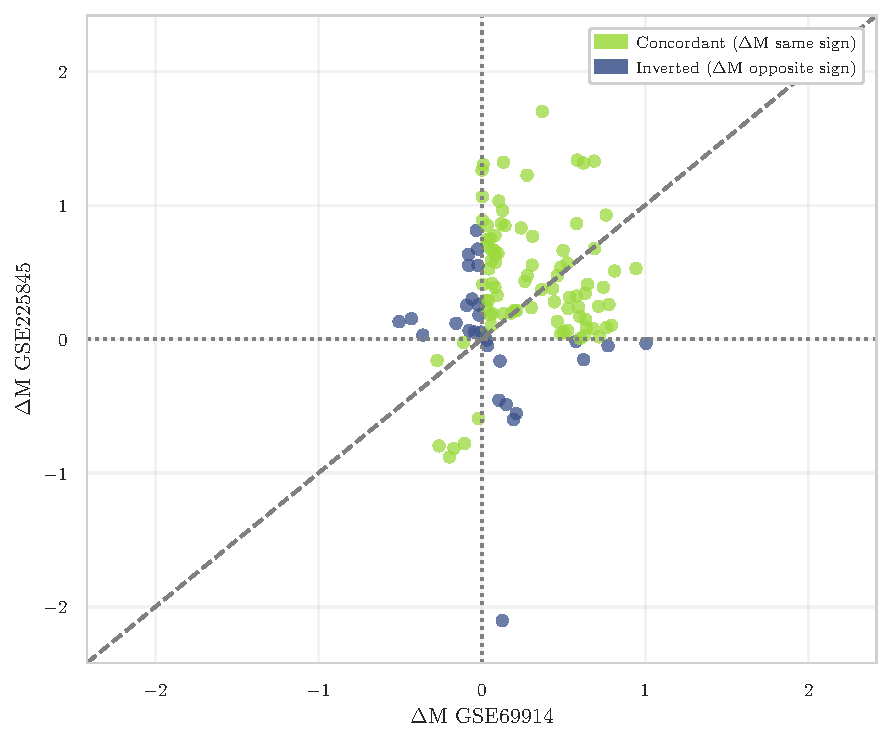
\includegraphics[width=\textwidth]
    {images/cap6/6x6_deltaM_scatter_GSE69914_vs_GSE225845.pdf}
  \caption{GSE69914 vs.\ GSE225845\\ ($\rho=0.08$, $c=0.76$).}
\end{subfigure}
\hfill
\begin{subfigure}[b]{0.31\textwidth}
  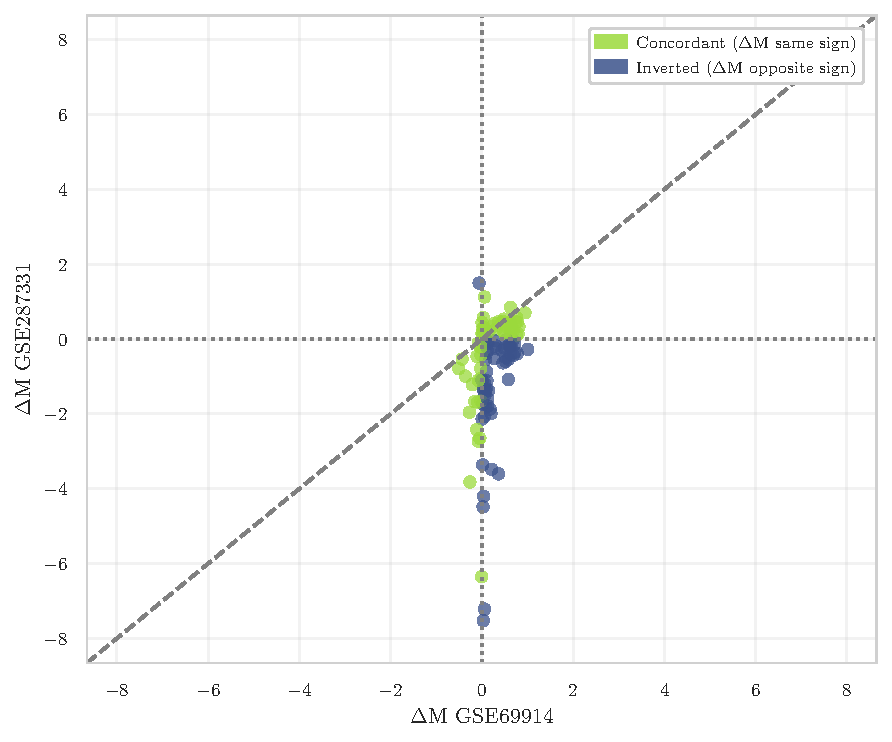
\includegraphics[width=\textwidth]
    {images/cap6/6x6_deltaM_scatter_GSE69914_vs_GSE287331.pdf}
  \caption{GSE69914 vs.\ GSE287331\\ ($\rho=0.49$, $c=0.50$).}
\end{subfigure}
\hfill
\begin{subfigure}[b]{0.31\textwidth}
  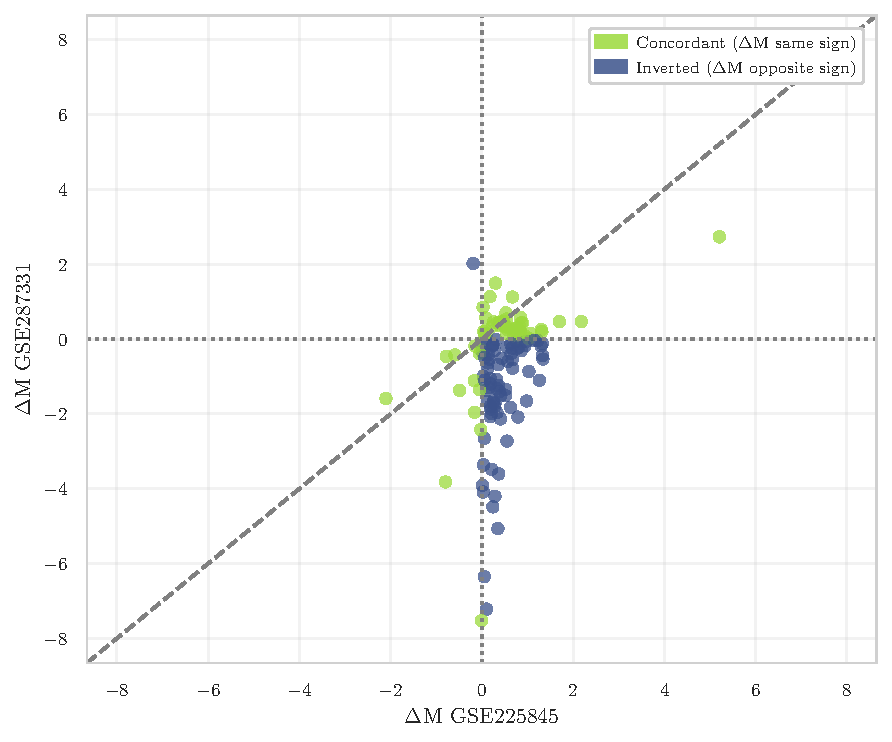
\includegraphics[width=\textwidth]
    {images/cap6/6x6_deltaM_scatter_GSE225845_vs_GSE287331.pdf}
  \caption{GSE225845 vs.\ GSE287331\\ ($\rho=0.38$, $c=0.42$).}
\end{subfigure}
\caption{Pairwise $\Delta M$ (Adjacent -- Normal) concordance
         scatter plots on the shared CpG intersection.
         Each point is one CpG; axes show the mean $\Delta M$
         computed independently in each cohort.}
\label{fig:deltam_scatter}
\end{figure}


\begin{figure}[H]
\centering
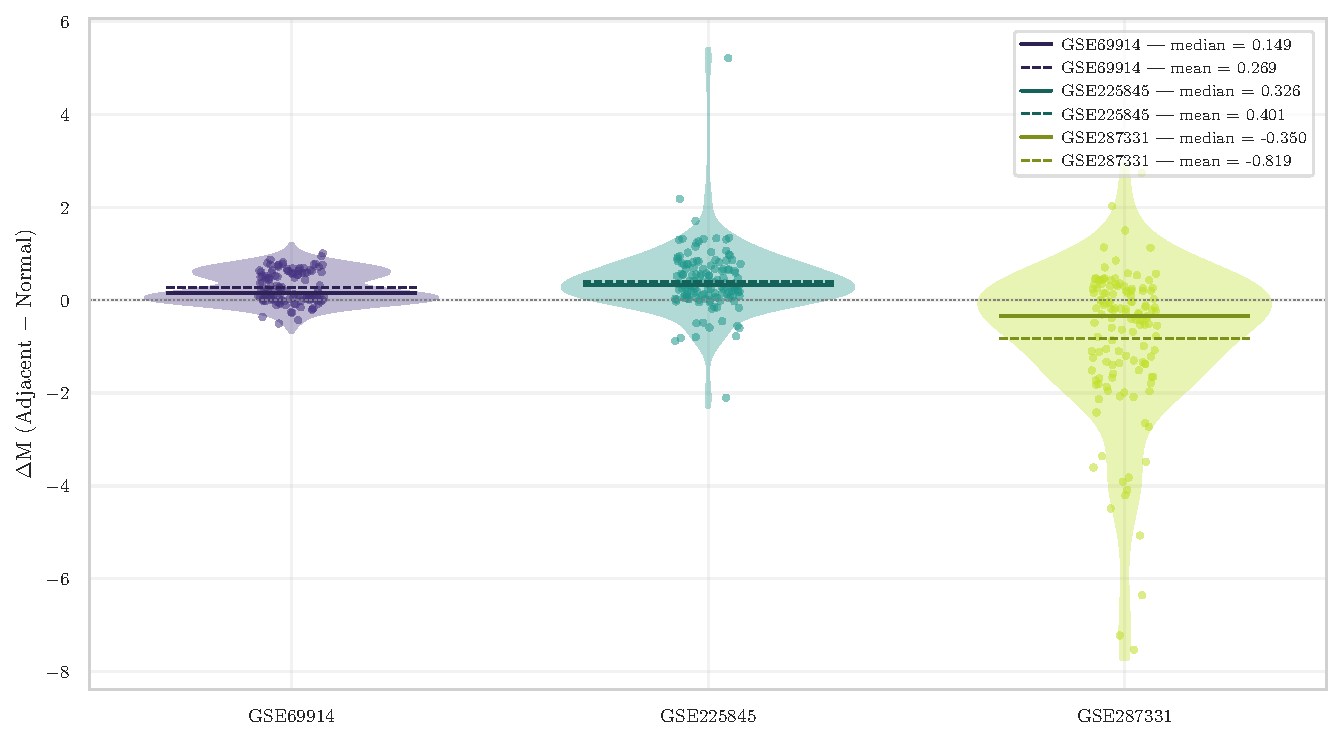
\includegraphics[width=0.65\textwidth]
  {images/cap6/6x6_deltaM_violin.pdf}
\caption{Distribution of $\Delta M$ (Adjacent -- Normal)
         across the three cohorts on the shared CpG
         intersection, stratified by sign-concordance group.}
\label{fig:deltam_violin}
\end{figure}

%-----------------------------------------------------------
\subsection{Synthesis and Implications for Joint Modelling}
\label{sec:inter_synthesis}
%-----------------------------------------------------------

The diagnostics of this section converge on three
structural properties of the joint methylation space.
First, biological signal is present in the leading variance
component of all three cohorts, confirming that the
Normal--Adjacent contrast is not an artefact of
preprocessing or selection. Second, dataset identity
dominates the joint variance structure, with batch-driven
PC1 AUC consistently matching or exceeding phenotype-driven
AUC; naive joint modelling in this space will absorb cohort
effects before biological signal. Third, the directional
structure of the drift is not uniformly conserved: GSE69914
and GSE225845 share a consistent drift orientation, whereas
GSE287331 exhibits systematic polarity inversion that
cannot be resolved by scaling or simple harmonisation.

Together, these findings establish that the failure of
cross-dataset transfer documented in
Section~\ref{sec:cross_dataset} reflects two distinct
obstacles: a dominant batch component that confounds the
joint feature space, and a structural orientation
asymmetry in GSE287331 that renders its drift axis
incompatible with a single shared linear representation.
Addressing both obstacles simultaneously requires an
approach that explicitly separates cohort variance from
phenotype variance while remaining agnostic to the
polarity of the drift direction. This motivates the
representation-learning strategy developed in
Chapter~\ref{chap:multi_cohort_integration}.

%-----------------------------------------------------------
\section{Synthesis and Implications}
%-----------------------------------------------------------

This section summarises predictive findings,
identifies structural limitations of linear
$\Delta\beta$-based signatures,
and motivates the transition toward
representation-learning approaches
in the subsequent chapter.